\documentclass[b5paper,draft,10pt,fleqn,twoside]{book}
% This TeX file is auto generated from a Org file.
% As such, is not properly documented.
% Please refer to the Org or HTML file instead for explanations.

\hfuzz1pc
\overfullrule=2cm

\usepackage[spanish,es-noindentfirst]{babel}
\usepackage{csquotes}

\usepackage[
	includehead,
	includefoot,
	letterpaper,
	top=2cm,
	bottom=2cm,
	left=4.5cm,
	right=4.5cm,
	marginparsep=0.5cm,
	marginparwidth=4cm,
]{geometry}

\usepackage{mathtools}
\DeclareMathOperator{\Rea}{Re}
\DeclareMathOperator{\Ima}{Im}
\DeclareMathOperator{\car}{car}
\DeclareMathOperator{\traz}{tr}
\DeclareMathOperator{\gen}{gen}
\DeclareMathOperator{\mcm}{mcm}

\usepackage{unicode-math}

\setmainfont{XCharter}
\defaultfontfeatures{Scale=MatchLowercase}
\setsansfont{TeX Gyre Heros}
\setmonofont{Go Mono}

\frenchspacing
\linespread{1.04}

\setmathfont{TeX Gyre Termes Math}

\usepackage[final]{microtype}

\PassOptionsToPackage{final}{graphicx}

\usepackage{%
	xcolor,%
	graphicx,%
	cancel,%
	booktabs,
	hyphenat,
	authoraftertitle,
	pdfpages,
	metalogo
}

\usepackage[
	backend=biber,
	backref=true,
	style=trad-abbrv,
	sorting=ynt
]{biblatex}
\addbibresource{/home/jhonny/git/Misc-LaTeX-files/bib/general.bib}

\usepackage{url} 
\usepackage{hyperref} 
\hypersetup{colorlinks=true,linkcolor=black,urlcolor=black}
\usepackage[spanish,nameinlink]{cleveref}

\usepackage{enumitem} 
\setlist[enumerate]{left=-11pt,nosep}
\setlist[description]{font=\normalfont,leftmargin=\parindent}
\setlist[itemize]{label={\small\textbullet},left=-11pt}

\usepackage[final]{listings} 
\lstset{
language=R, 
numbers=left, numberstyle=\tiny\ttfamily, stepnumber=2, numbersep=5pt, 
basicstyle=\ttfamily, 
stringstyle=\ttfamily,
commentstyle=\itshape,
breaklines=true,
postbreak=\mbox{$\hookrightarrow$\enspace},
columns=flexible
}

\usepackage{caption} 
\captionsetup{
font={rm},
justification=raggedright,
singlelinecheck=false,
skip=3pt
}

\usepackage[explicit]{titlesec}

\titleformat{\part}[display]
{\flushleft\sffamily\fontsize{40}{40}\selectfont}
	{\thepart}
	{3em}
	{#1}
	[]
\titleformat{\chapter}[display]
	{\flushleft\Large\sffamily}
	{\large\thechapter}
	{1em}
	{#1}
	[]
\titlespacing*{\chapter}
	{0em}
	{0em}
	{3\baselineskip}
\titleformat{\section}[hang]
	{\flushleft\sffamily}
	{\hspace{-2.4em}\S\thesection}
	{.5em}
	{\MakeUppercase{#1}}
	[]
\titlespacing*{\section}
	{0em}
	{1.5\baselineskip}
	{0\baselineskip}
\titleformat{\subsection}
	{\flushleft\sffamily}
	{\thesubsection}
	{.5em}
	{#1}
	[]
\titlespacing*{\subsection}
	{0em}
	{1\baselineskip}
	{0\baselineskip}

\usepackage{titletoc}

\titlecontents{part}
[1em]
{\vspace{.3em}}%
{\large\contentsmargin{0pt}}
{\large\contentsmargin{0pt}}
{}                 		
[\vspace{4pt}]
\titlecontents{chapter}
[1em]
{\vspace{.3em}}%
{\contentsmargin{0pt}}
{\contentsmargin{0pt}}
{\hspace{3pt}\contentspage}                 		
[\vspace{4pt}]
\titlecontents{section}
[4em]
{}
{\contentsmargin{0pt}}
{\contentsmargin{0pt}}
{\hspace{3pt}\contentspage}
[\vspace{5pt}]
\titlecontents{subsection}
[5.5em]                              
{\vspace{-4pt}}
{\contentsmargin{0pt}\small\enspace}
{\contentsmargin{0pt}}        
{\small\contentspage}                 
[\vspace{3pt}]

\usepackage{fancyhdr}

\renewcommand{\headrulewidth}{0pt}
\setlength{\headheight}{14pt}

\pagestyle{fancy}
\renewcommand{\chaptermark}[1]{%
	\markboth{#1}{}}
\renewcommand{\sectionmark}[1]{\markright{#1}}
\fancyhead[R]{\ifodd\value{page}{\nouppercase\rightmark}\else{}\fi}
\fancyhead[L]{}
\fancyfoot[R]{\thepage}
% \fancyhead[OL]{\sffamily\nouppercase\rightmark}
% \fancyhead[EL]{\sffamily\thepage}
% \fancyhead[ER]{\sffamily\nouppercase{\leftmark}}
% \fancyhead[OR]{\sffamily\thepage}
\fancyfoot[L]{}
\fancyfoot[C]{}
\fancypagestyle{plain}{%
	\fancyhead[R]{}
	\fancyhead[L]{}
	\fancyfoot[R]{}%
	\fancyfoot[L]{}
	\fancyfoot[C]{}
}

\usepackage[thmmarks]{ntheorem}
	\theoremstyle{plain}
	\theoremindent0cm
	\theorempreskip{0cm}
	\theorempostskip{0cm}
	\theoremheaderfont{\hspace*{\parindent}\upshape}
	\theorembodyfont{\itshape}
	\theoremseparator{.}
	\newtheorem{teo}{Teorema}[section]
	\newtheorem{cor}{Corolario}[teo]
	\newtheorem{prop}{Proposición}[section]
	\newtheorem{lem}{Lema}[section]
	\theoremstyle{nonumberplain}
	\theoremheaderfont{\normalfont}
	\theorembodyfont{\upshape}
	\newtheorem{proof}{Demostración}
	\theoremstyle{plain}
	\theoremheaderfont{\upshape}
	\theorempostwork{\noindent}
	\newtheorem{definition}{Definición}[section]


\begin{document}
% Pagina de titulo
\frontmatter
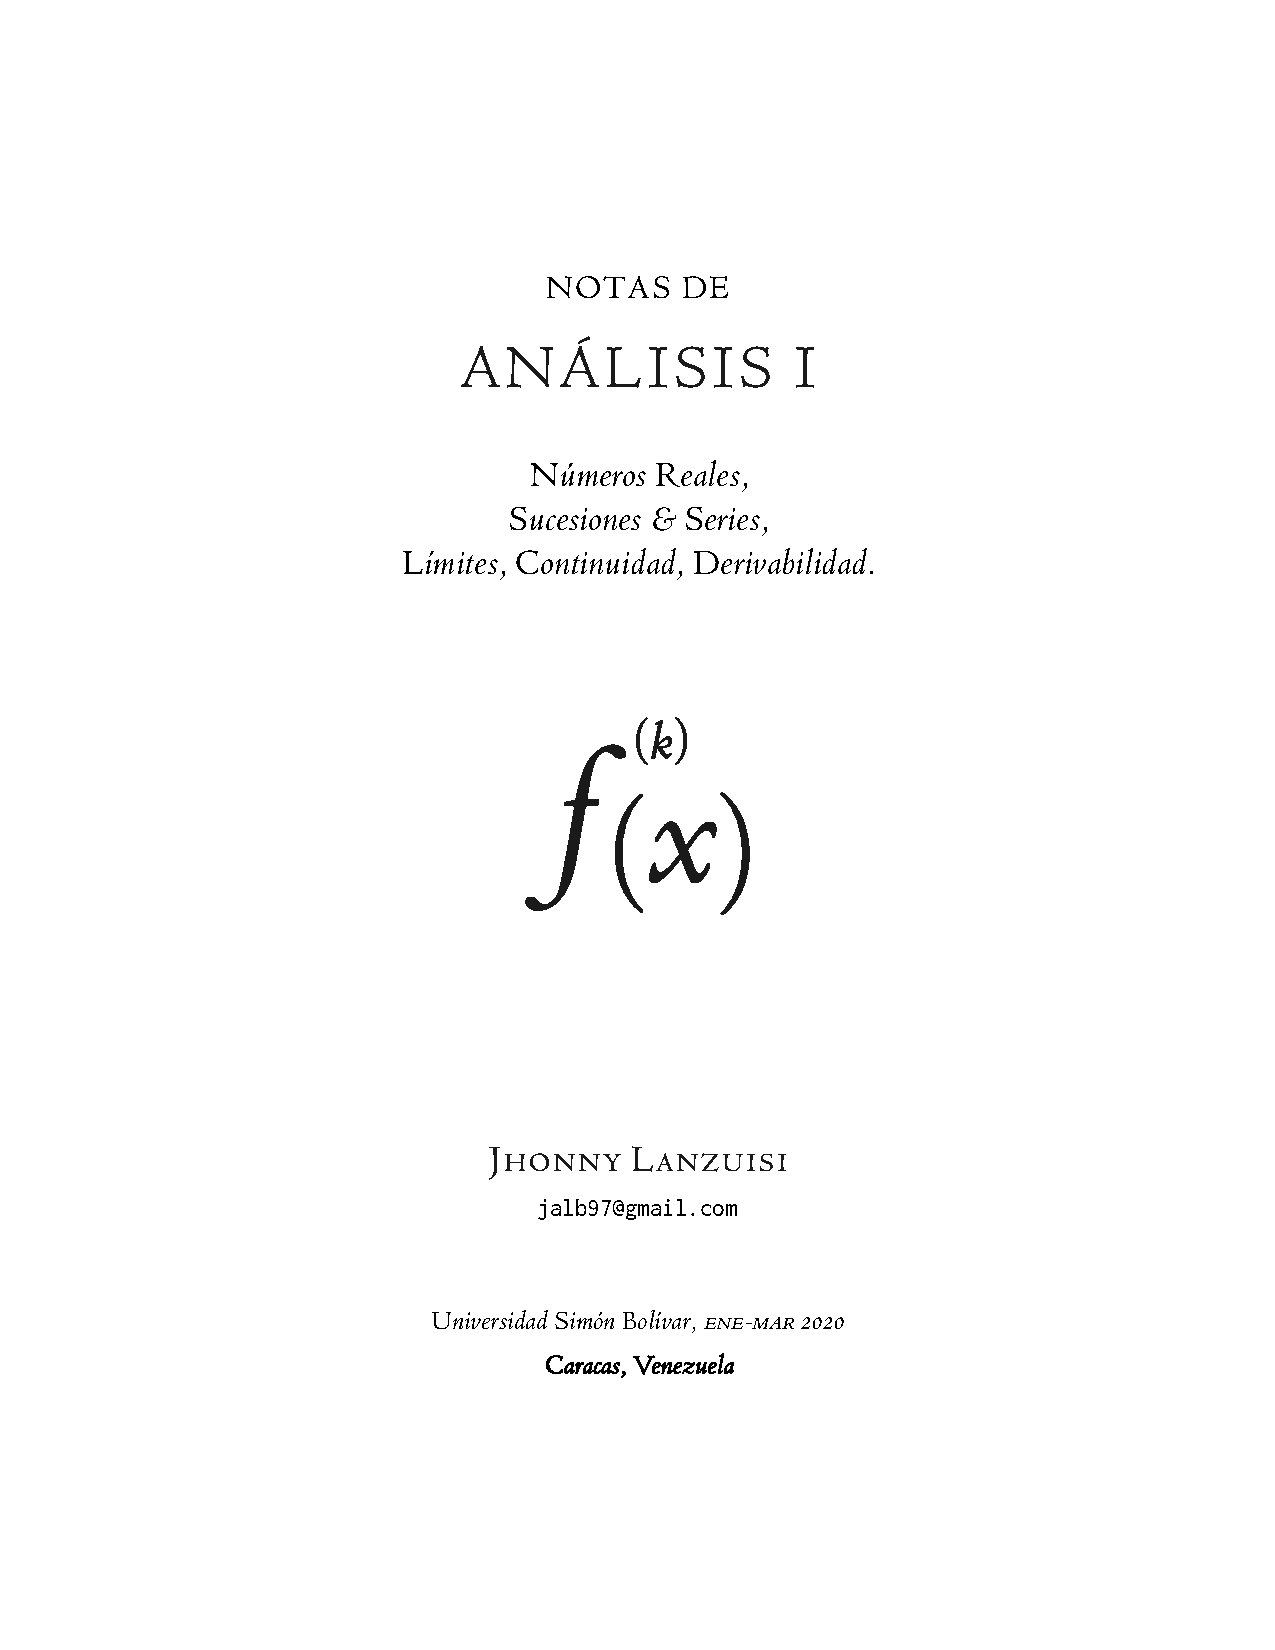
\includepdf[pages=-]{portada.pdf}
\clearpage
% Indice
\tableofcontents
% Prefacio
%\thispagestyle{plain} 
%\setcounter{page}{1} \pagenumbering{roman}
\chapter{Prefacio}%
\label{cha:Prefacio}


{\noindent Estas notas cumplen un doble propósito: ser de ayuda a cualquier infortunado que se tope con ellas y servir como material de estudio a su autor. }

Comenzando como una introducción a la teoría de Anillos, basado en el curso que se dicta en la USB\footnote{Universidad Simón Bolívar.}, estas notas han ido creciendo hasta convertirse en lo que son hoy: una introducción al álgebra abstracta, desde los conceptos más básicos de la teoría de conjuntos y relaciones hasta la teoría de anillos. 

Los prerrequisitos para leer el texto, siendo este una introducción, son mínimos. Dicho esto, no vendría mal haber visto alguna vez un poco de matemáticas `abstractas' o `rigurosas': como los argumentos de `epsilon-delta' que se dan en un curso usual de cálculo, o las demostraciones axiomáticas típicas de un curso sobre geometría euclídea. En cualquier caso, lo anterior no es en absoluto un requisito por lo que el lector que no esté acostumbrado a estos temas no debe temer: este libro también es para el.

\marginnote{Los comentarios en el texto estarán en este formato. El lector es libre de ignorarlos, a veces serán referencias históricas, otras veces sugerencias.}
%Con respecto al primero de estos propósitos, los contenidos serán mas o menos los del curso `Introducción a la teoría de anillos' que se da en la USB\footnote{Universidad Simón Bolívar.}. Si el lector no es de los que tienen la fortuna (o quizás la desgracia) de estar viendo este curso, su propósito educativo es muy claro: servir de introducción a la teoría de anillos. En este sentido, se presupone cierta comodidad con los conceptos de la teoría de grupos\footnote{Que se pueden consultar en el herstein\cite{topicsinalgebra}}.

Se podrán encontrar una variedad de ejercicios de distintas fuentes, los de ellos que estén resueltos, lo están con la intención de que el lector los intente por su cuenta antes de ver la resolución propuesta. Evidentemente las respuestas dadas no serán las mas elegantes, en cuyo caso se insta al lector a enviar aquellas resoluciones que el o ella\footnote{O como el lector prefiera identificarse, no quiero ser acusado de lógica binaria.} considere mejores que las aquí presentes, al correo \url{jalb97@gmail.com}. 
%
Por último, las referencias podrán encontrarse al final del texto. 
 
% Introduccion
\thispagestyle{plain}
\chapter{Introducción}%
\label{cha:Introducción}

{\noindent Aunque no es estrictamente necesario, sería bueno tener algo de conocimiento sobre la teoría de grupos, en la cual se estudian las propiedades generales de un conjunto con una sola operación binaria.}

Nos interesa ahora pensar el caso de las estructuras algebraicas que poseen dos operaciones binarias, sus propiedades y sus aplicaciones. En este sentido, el lector no deberá sorprenderse al ver que comenzamos nuestro estudio de forma análoga al estudio de la teoría de grupos, hablando de subanillos, anillos cocientes, ideales (que son el equivalente de los subgrupos normales) y homomorfismos de anillos. En lo que concierne a la nueva operación binaria introducida, el \textit{producto}, su estudio nos llevará al concepto de Cuerpo y eventualmente a construcciones mas específicas como los cuerpos finitos.

% Numeros normales de pagina
\mainmatter
\part{Teoría de Conjuntos}
%\input{../../Plantillas-Fomato/Libros/Libro-Anillos.tex}
\thispagestyle{plain}

\chapter{Introducción a los Conjuntos}
\epigraph{En matemáticas el arte de hacer preguntas es más valioso que resolver problemas}{georg cantor}

\noindent El concepto central de este capítulo ---y pieza fundamental en la matemática moder\-na--- es, al menos en la superficie, tremendamente simple. Un \textit{conjunto} es un agregado de objetos, una colección o grupo de estos objetos. Así, tenemos que la colección de los estudiantes inscritos en la Universidad Simón Bolívar es un conjunto, como también lo es la cantidad de dígitos en la expansión decimal de $\pi$.
 	
\marginnote{Esta noción de conjunto, en principio simple e intuitiva, irá revelando su dificultad a medida que se resuelvan problemas y se avance un poco en los conceptos.
}
Los conjuntos son una construcción abstracta, pensada por una cabeza humana, que consiste en agrupar todos los objetos que cumplen con una cierta propiedad. Esta propiedad puede ser en principio cualquiera, aunque más adelante daremos formas precisas de enunciar las propiedades para no caer en ambigüedades. Entonces todos los números que tienen la propiedad de ser múltiplos de dos son un conjunto, como también lo es la colección de todos los hijos que son a la vez sus propios padres (este último conjunto, aparentemente contradictorio, es \textit{vacío}. La noción de vacío se verá mejor más adelante).

Es interesante notar que, si nos conformamos con la definición que hemos dado hasta ahora y la tomamos como definitiva, pueden surgir contradicciones e inconsistencias. Quizás el ejemplo mas paradigmático es el siguiente, dicho en la versión del mismo que el autor de esta guía escuchó por primera vez.

\begin{ejem}[Paradoja de Russel\footnotemark]
	Existe un pueblo, en una tierra muy lejana, donde trabaja un solo barbero. Pero este barbero tiene una exigencia peculiar a sus clientes: solo afeita a aquellos que no se afeitan a ellos mismos. Todo estaría bien con nuestro barbero si no se nos ocurriese la siguiente pregunta: ¿El barbero se afeita a si mismo?
	
	Veamos. Si el barbero se afeita a si mismo entonces, por la \textit{propiedad} especial que cumple nuestro barbero, se sigue que el barbero no se afeita a si mismo: una contradicción. De igual forma, si el barbero no se afeita a si mismo entonces el babero sería una persona que no se afeita a si misma y tendríamos, por la condición peculiar de nuestro barbero, que se afeita a si mismo: otra contradicción.
	 		
	Tenemos que, sin importar que respuesta demos a nuestra pregunta, siempre llegamos a una contradicción: una paradoja. Los sistemas que se comportan de esta forma se suelen llamar \textit{inconsistentes}.
	
	La paradoja de Russel puede formularse formalmente, utilizando notación que no hemos explicado aún, de la siguiente manera: Sea $R = \{ x \mid x \notin x \}$ preguntémonos si $R\in R$. Se deja como un ejercicio al lector volver después de la siguiente sección y desarrollar la paradoja de Russel en lenguaje formal.
\end{ejem}
\footnotetext{Bertrand Russel fue un matemático británico del siglo \textsc{xx} que trabajó mucho en el área de filosofía de las matemáticas.}
La lección que se saca de ejemplos como la paradoja de Russel es que el conjunto nombrado no existe y que, en general, ser capaz de nombrar un conjunto no es condición suficiente para asegurar su existencia. Más aún, no tenemos hasta ahora ninguna manera de definir formalmente la noción de conjunto de tal forma que contradicciones como las del ejemplo anterior no ocurran. Por esta razón es que no intentaremos dar una noción mas formal de la idea de conjunto, en cambio daremos unos cuantos \textit{axiomas} que describen bastante bien como esperamos que se comporte un conjunto. Y partiendo de estos axiomas construiremos el resto de nuestra teoría.

Un \textit{axioma} es una verdad que asumiremos sin demostración.

\section{Propiedades}

En nuestra definición de conjunto aludimos a unas \textit{propiedades} que los elementos del conjunto compartían. Tenemos ahora la tarea de establecer ciertas reglas con las que podamos enunciar estas propiedades, con el fin de evitar ambigüedades. 

Las reglas que vamos a explicar son, en esencia, las de la \textit{lógica}. Si se quiere un estudio riguroso de estas reglas será mejor remitirse a un libro de lógica matemática, aquí se hablará de los conceptos de manera informal.

La relación más básica en la teoría de conjuntos es la de \textit{pertenencia}, que denotamos con el símbolo $\in$. La expresión $X\in Y$ se lee `$X$ pertenece a $Y$' o `$X$ es un miembro de $Y$'.

Las letras $X$ e $Y$ usadas en el párrafo anterior son \textit{variables}, denotan cualquier par de conjuntos. La proposición `$X\in Y$' es verdadera o falsa dependiendo de cuales son los conjuntos $X$ e $Y$.

Todas las demás propiedades de la teoría de grupos se pueden expresar usando la pertenencia y algunas herramientas lógicas: identidad, conectividad y cuantificadores.

Hay veces en las que conviene expresar el mismo conjunto con variables distintas, la relación de igualdad ---o identidad--- de conjuntos la denotaremos con el símbolo `$=$'.

\begin{ejem}
	Este ejemplo da varios hechos sobre la igualdad de conjuntos. Sean $X,Y$ y $Z$ tres conjuntos, entonces se cumple que:
	\begin{enumerate}
		\item $X=X$.
		\item Si $X=Y$ entonces $Y=X$.
		\item Si $X=Y$ y $Y=Z$, entonces $X=Z$. 
		\item Si $X=Y$ y $X\in Z$ entonces $Y\in Z$.
		\item Si $X=Y$ y $Z\in X$ entonces $Z\in Y$.
	\end{enumerate}
\end{ejem}

\part{Teoría de Grupos}
\part{Teoría de Anillos}
% Primera seccion
%\vspace*{5em}
%\input{../../Plantillas-Fomato/Libros/Libro-Anillos.tex}

\chapter{Definiciones Básicas y Ejemplos} 
\epigraph{Comunmente en las matemáticas el problema crucial es reconocer y descubrir cuales son los conceptos relevantes, una vez hecho esto esta casi la mitad del trabajo listo}{i. n. herstein}

{\noindent Nuestro punto de partida, y la pieza central la teoría de anillos, es la siguiente definición.}

\begin{defi}[anillo]
	Un anillo $\an{A}$ es un conjunto con dos operaciones binarias, $+$ y $\t$ (llamadas suma y producto), que satisface, para todo $a,b,c$ en $\an{A}$,
	\begin{enumerate} 
		\item $(\an{A},+)$ es un grupo abeliano.
		\item El producto es asociativo: $(a \t b) \t c = a \t (b \t c)$
		\item Se cumple la propiedad distributiva:
		\begin{align*}
		(a+b) \t c &= (a\t c) + (b\t c) \quad \text{y,} \\
		c\t (a+b)  &= (c\t a) + (c\t b).
		\end{align*} 
	\end{enumerate}
\end{defi}
\begin{nota}
	Los anillos fueron desarrollados a principios del siglo \textsc{xix}, aunque no fue hasta el segundo tercio del siglo \textsc{xx} que adquirieron notoriedad.
\end{nota}
%
Cabe destacar que, las operaciones suma y producto antes descritas son abstractas, y no son aquellas a las que estamos acostumbrados en, por ejemplo, el conjunto $\R$ de los números rea\-les. Otra acotación importante es que, de acuerdo con la definición anterior, siempre que se hable de un anillo $\an A$ deben especificarse las operaciones junto con a las cuales $\an A$ forma un anillo. Los momentos en los que se omitan estas operaciones serán solo los casos en que sean evidentes.

Diremos que un anillo $\an A$ es \textit{conmutativo} cuando, como cabría esperar, el producto sea conmutativo. Además, si $\an A$ posee un elemento $1$ tal que $1 \t a = a\t 1 = a$, para todo $a \in\an A$, diremos que $\an A$ es  unitario.

A partir de ahora, adoptaremos las siguientes convenciones. Sea $\an A$ un anillo. El producto $a\t b$ se denotará simplemente como $ab$, para cuales quiera elementos $a,b \in\an A$. La identidad aditiva será denotada por $0$ y el inverso aditivo (\textit{opuesto}) de un $a \in\an A$ será denotado por $-a$. Estas convenciones son familiares del conjunto $\Z$ de los enteros.

 La condición de que $\an A$ sea un grupo bajo la adición es natural, por otro lado, la condición de que sea abeliano puede parecer un poco forzada. Una de la razones principales de que se le pida una condición tan restrictiva es que, si el anillo es unitario, entonces la conmutatividad de la suma se ve \textit{forzada} por la propiedad distributiva. 

\begin{nota}
	Para ver esto, se calcula $(1+1)(a+b)$ de forma artificiosa.
\end{nota}
%
 Un anillo $\an A$ unitario (con $1 \neq 0$) es llamado de \textit{división} si todo elemento no nulo $a$ de $\an A$ posee un inverso multiplicativo, es decir, si para todo $a \in\an A$ existe un $b \in\an A$ tal que $ab = ba = 1$. Ahora podemos considerar la siguiente definición. 

\begin{defi}[cuerpo]  
	Un cuerpo es un anillo de división conmutativo.
\end{defi} 
\begin{nota}
	Los angloparlantes prefieren la palabra \textit{Campo (Field)} en vez de \textit{Cuerpo}.
\end{nota}
Es un ejercicio interesante, aunque quizás tedioso, desglosar la definición anterior y darla en función de las propiedades nombradas. A continuación, más ejemplos.
\begin{ejem}
	Los ejemplos más sencillos de anillos son los anillos \textit{triviales} formados tomando cualquier grupo conmutativo $\an A$ con el siguiente producto trivial, para todo $a,b \in\an A$, $ab=0$. Es fácil revisar que este $\an A$ es un anillo conmutativo. En el caso de que $\an A=\{0\}$ se obtiene el \textit{anillo cero}, denotado por $\an A=\an0$. 
\end{ejem}
\begin{ejem} 
	El conjunto de los enteros, $\Z$, bajo las operaciones usuales de suma y producto es un anillo conmutativo con identidad, pero \textit{no} un cuerpo. ¿Cuáles son los elementos de $\Z$ invertibles, es decir, con inverso multiplicativo?
\end{ejem}
\begin{ejem}
	Los conjuntos $\Q$ y $\R$, de los racionales y los reales, son anillos conmutativos con unidad (¿Son cuerpos?). 
\end{ejem}
\begin{ejem}
	El grupo cociente $\Zn$ es un anillo conmutativo con identidad al usar el producto \textit{módulo n}, de las clases de equivalencia, esto es, el producto de dos elementos es la clase de su multiplicación usual. 
\end{ejem} 
%
Los ejemplos dados hasta ahora han sido todos de anillos conmutativos, los anillos no conmutativos son también un área importante del álgebra, en este sentido se tiene el siguiente ejemplo. 

\begin{ejem}[Cuarteniones Hamiltonianos] 
	Sea $\Ha$ el conjunto de los elementos de la forma $a + bi + cj + dk$, donde $a,b,c,d \in \R$, con la suma definida `por componentes':
	\begin{align*}
	(a + bi + &cj + dk)+(a' + b'i + c'j + d'k) = \\ (&a+a') + (b+b')i + (c+c')j + (d+d')k 
	\end{align*}
	y el producto definido expandiendo $(a + bi + cj + dk)(a' + b'i + c'j + d'k)$ de acuerdo con la propiedad distributiva.  El producto se hace tomando en cuenta que
	\[  i^2=j^2=k^2=-1 \]
	junto con las siguientes reglas multiplicativas
	\[ ij=-ji=k, \; jk=-kj=i, \; ki=-ik=j, \]
	y que los números reales conmutan con los elementos $i,j,k$. De las relaciones anteriores es claro que los cuaterniones son en efecto no conmutativos. 
\begin{nota}
	El lector acostumbrado a la teoría de espacios vectoriales se habrá dado cuenta que los cuaterniones, así definidos, representan un espacio 4-di\-mensional sobre $\R$ con los vectores $\{1,i,j,k\}$ como base.
\end{nota}
	El hecho de que los cuaterniones son un anillo se puede ver mediante un chequeo, bastante tedioso, de las propiedades. Nótese que el elemento identidad es $1 + 0i + 0j +0k$. Más aún, los cuaterniones son un anillo no conmutativo de división, donde el inverso de un elemento ---no nulo--- viene dado por  
	\[ (a + bi + cj + dk)^{-1} = \frac{a - bi - cj - dk}{a^2+b^2+c^2+d^2}. \]
\end{ejem} 
\begin{nota}
	El álgebra no conmutativa se empezó a desarrollar en el siglo diecinueve de la mano de matemáticos como  W. R. Hamilton\footnotemark, I. N. Herstein, entre otros.
\end{nota}
\footnotetext{Sir William Rowan Hamilton (1805--1865) fue un matemático irlandés conocido por aportes importantes en las áreas de óptica, mecánica clásica y álgebra.}
Se pueden obtener ejemplos interesantes de anillos considerando anillos de funciones, como lo muestra el siguiente ejemplo.
\begin{ejem} \label{ejemap} 
	Sea $X$ un conjunto no vació y $\an A$ un anillo. La colección, $\an F$, de todas las funciones $f\mathpunct{:} X \to\an A$
	es un anillo con las operaciones usuales: 
	\[ (f+g)(x) = f(x)+g(x) \quad \text{y} \quad (fg)(x) = f(x)g(x). \]
	%
	El hecho de que $\an F$ sea un anillo se hereda directamente de $\an A$. Más aún, $\an F$ es conmutativo si, y solo si, $\an A$ lo es y $\an F$ tiene un $1$ si, y solo si, $\an A$ tiene un $1$ (en cuyo caso el $1$ de $\an F$ es necesariamente la función constante $f(x)=1$).
	
	Si $X$ y $\an A$ poseen estructuras con mas propiedades, se pueden formar anillos mas complejos. Por ejemplo, si tomamos $\an A$ como el anillo de los números reales y tomamos $X$ como el intervalo cerrado $[0,1]$ de $\R$, obtendremos el \textit{anillo de las funciones continuas}, el cual es conmutativo y posee un $1$.  
\end{ejem}
\begin{nota}
	Aunque sea tedioso, puede ser útil para el lector verificar todo lo que se afirma en el ejemplo anterior sobre los anillos de funciones.
\end{nota}
Puede ocurrir también que un anillo no posea identidad.
\begin{ejem}
	El anillo $2\Z$ de los números pares, bajo la multiplicación y la suma usuales, es un anillo conmutativo \textit{sin} identidad.
\end{ejem}
%
El siguiente teorema nos dará unas cuantas propiedades de los anillos que son familiares del conjunto $\Z$. 

\begin{teo} 
	Sea $A$ un anillo. Entonces, para todo $a,b \in A$, 
	\begin{enumerate}
		\item $0a=a0=0$ 
		\item $(-a)b=a(-b)=-(ab)$ 
		\item $(-a)(-b)=ab$ 
		\item Si $1\in A$ es una identidad, entonces esta identidad es \textit{única} y $-a=-1(a)$
	\end{enumerate} 
\end{teo}
\begin{nota}
	En la siguiente demostración, como en muchas otras, la clave esta en pensar cuidadosamente en las propiedades que poseen los objetos con que estamos trabajando. Por ejemplo, para probar (2), se quiere ver que ese elemento actúa como inverso aditivo de $(ab)$.
\end{nota}
\begin{proof}
	El teorema se sigue de la propiedad distributiva y de la ley de cancelación (considerando a $A$ como un grupo aditivo). Veamos cada una, para todo $a,b\in A$, 
	\begin{enumerate}
		\item $0a = (0+0)a = 0a + 0a$ de donde, por la ley de cancelación, $0a=0$. Igualmente para $a0=0$.
		\item Primero, $ab + (-a)b = (a+(-a))b = 0b = 0$ y por otro lado $ab + a(-b) = a(b+(-b)) = a0 = 0$. 
		\item Por la parte anterior, $(-a)(-b) = -(-ab) = ab$.
		\item Supongamos que existe un $1'$ tal que $1'a = a1' = a$ entonces ocurriría que $(1')1 = 1$ y $(1')1 = 1'$, lo cual es imposible, luego solo existe un elemento identidad en $A$. Por 2, $-a = 1(-a) = (-1)a$.
	\end{enumerate}
\end{proof}
%
\section{Dominios enteros y divisores de cero}
A diferencia del conjunto $\Z$, puede ocurrir que en un anillo existan elementos no nulos $a,b$ tales que $ab=0$. Esto motiva la siguiente definición. 
\begin{defi}[divisor de cero] 
	Sea $A$ un anillo, 
	\begin{enumerate}
		\item Un elemento no nulo $a$ de $A$ es un \textit{divisor de cero} si existe un $b \in A$, no nulo, tal que $ab = 0$ o $ba = 0$.
		\item Supongamos que $A$ posee una identidad $1$, con $1 \neq 0$. Un elemento $v \in A$ es llamado una \textit{unidad} si existe un $w \in A$ tal que, $vw = wv = 1$. El conjunto de las unidades de $A$ se denota por $A^{\t}$.
	\end{enumerate}
\end{defi}
\begin{nota}
	Los divisores de cero nos son familiares de las matrices reales.
\end{nota}
En la terminología de la definición anterior, un anillo $A$ es un cuerpo si todos los elementos no nulos son unidades, o lo que es lo mismo, si $A^{\t}=  A - \{0\}$. 

Nótese que un divisor de cero no puede ser una unidad. En efecto, supongamos que $a \in A$ es una unidad tal que existe un $b \in A$, no nulo, para el cual $ab = 0$. Entonces, como $a$ es una unidad, existe un $v \in A$ tal que $va = 1$, de donde se sigue que $b = 1b = (va)b = v(ab) = 0$, lo cual es una contradicción. Lo mismo ocurre si $ba = 0$. Una consecuencia de esto es que \textit{en un cuerpo no hay divisores de cero.}

Continuamos con ejemplos, esta vez sobre divisores de cero y unidades.
\begin{ejem}
	El anillo $\Z$ de los enteros no posee divisores de cero, y sus únicas unidades son $\pm 1$, es decir, $\Z^{\t} = \{-1,1\}$.
\end{ejem}
\begin{ejem} 
	Si $A$ es el anillo de todas las funciones que van del intervalo cerrado $[0,1]$ a $\R$ entonces sus unidades son todas las funciones que no se anulan en ningun punto (para esta clase de funciones su inverso viene dado por $1/f$). Si $f$ no es una unidad y tampoco se anula, entonces $f$ es un divisor de cero. Esto se debe a que podemos definir la siguiente 
	\[ g(x) = \begin{cases}
	\hspace{.5em} 0  \quad \text{si} \; f(x) \neq 0 \\ 
	\hspace{.5em} 1 \quad \text{si} \; f(x) = 0
	\end{cases} \]
	que no se anula, sin embargo, $f(x)g(x) = 0$ para todo $x$.
\end{ejem} 
\begin{nota}
	Siempre que se quiera que una función cumpla un papel específico, y no se le ocurra ninguna ¡defínala por partes!
\end{nota}
A los anillos que se parecen mucho a los enteros se les da un nombre especial.

\begin{defi}[dominio entero] 
	Un anillo conmutativo con identidad es un dominio entero si no posee divisores de cero.
\end{defi}
%
El hecho de que no existan divisores de cero hace que los dominios enteros posean una ley de cancelación, como explica el siguiente teorema.
\begin{teo}
	Supongamos que $a,b$ y $c$ son elementos de un anillo y que $a$ no es un divisor de cero. Si $ab=ac$ entonces se tiene que $a=0$ o $b=c$.
\end{teo}
\begin{proof}
	Si $ab = ac$ entonces $a(b-c) = 0$ de donde se sigue que $a = 0$ o $b-c = 0$. 
\end{proof} 
\begin{cor}
	Todo dominio entero finito es un cuerpo.
\end{cor} 
\begin{proof}
	Sea $A$ un dominio entero finito y sea $a$ un elemento, no nulo, de $A$. La función $f\mathpunct{:}A \to A$ definida por $f(x) = ax$ es inyectiva, debido a la ley de cancelación. Como $A$ es finito esta función es sobreyectiva. En particular, existe un $b \in A$ tal que $ab=1$, es decir, $a$ es una unidad en $A$. Como lo anterior es cierto para \textit{cualquier} $a \in A$, se sigue que $A$ es un cuerpo.
\end{proof}
%
\section{Subanillos}
\noindent Es natural considerar la noción de \textit{subanillo}. 

\begin{defi}[subanillo] 
	Un subanillo, de un anillo $A$, es un subgrupo de $A$ que es cerrado bajo el producto. 
\end{defi}
\begin{nota}
	También se puede pensar que un subanillo es un subconjunto que tiene el también estructura de anillo.
\end{nota}
%
De la definición anterior se sigue que, para mostrar que un conjunto es un subanillo, hace falta ver que es \textit{no vacío} y \textit{cerrado bajo la diferencia y el producto}.

Continuamos con más ejemplos, esta vez de subanillos.
\begin{ejem}
	$\Z$ es un subanillo de $\Q$ y $\Q$ es un subanillo de $\R$. La propiedad `ser un un subanillo de' es claramente transitiva.
\end{ejem} 
\begin{ejem} 
	$2\Z$ es un subanillo de $\Z$, de la misma forma, $n\Z$ es un sub\-anillo de $\Z$ para todo $n$.
\end{ejem}
\begin{nota}
	Es un ejercicio rápido verificar el ejemplo anterior
\end{nota} 
\begin{ejem}
	El anillo de todas las funciones continuas de $\R$ en $\R$ es un sub\-anillo del anillo de las funciones de $\R$ en $\R$. El anillo de las funciones \textit{diferenciables} es un subanillo de los dos.
\end{ejem} 
\begin{ejem}
	Los \textit{cuaterniones enteros}, es decir, los elementos de la forma $a+bi+cj+dk$ con $a,b,c,d \in \Z$, son un subanillo de los cuaterniones reales o racionales.
\end{ejem}
\begin{nota}
	Las subestructuras son muy comunes en el álgebra. El lector podrá pensar en muchos ejemplos, como los subgrupos o los subespacios.
\end{nota}
\begin{ejem}
	Si $A$ es un subanillo, de un cuerpo $C$, que contiene a la identidad de $C$, entonces $A$ es un dominio entero. El converso también es cierto, todo dominio entero esta contenido en un cuerpo.
\end{ejem} 
\section{Potencias y múltiplos}
\noindent Las nociones de múltiplo y de potencias a las que estamos acostumbrados tienen una generalización natural en los anillos.

Sea $a$ un elemento de un anillo $A$ y $n \in \N$. Entonces la \textit{enésima potencia} de $a$, $a^n$, se define mediante las condiciones inductivas  
\[ a^1=a \quad \text{y} \quad a^n=a^{n-1}a \] 
de esto las reglas usuales se los exponentes se siguen directamente:
\[ a^na^m=a^{n+m}, \quad (a^n)^m = a^{nm}, \quad (n,m \in \N). \]
Nótese que si dos elementos, $a,b$, conmutan, entonces sus potencias también lo hacen y $(ab)^n = a^nb^n$. 

En el caso de que $A$ sea unitario y $a^{-1}$ exista, se pueden considerar \textit{potencias negativas} de $a$ definidas mediante la siguiente expresión
\[ a^{-n} = (-a)^n, \]
que junto con la definición de $a^0=1$, nos dan una definición de las potencias para todo elemento de $\Z$.


Consideramos ahora el caso de los múltiplos. Para cada $n \in \Z$ definimos el \textit{múltiplo enésimo} de $a$, $na$, de manera recursiva:
\[ 1a=a \quad \text{y} \quad na=(n-1)a+a, \quad \text{cuando} \; n>1. \]
%
Si definimos $0a=0$ y $(-n)a = -(na)$ entonces la definición de múltiplo queda bien definida para cualquier entero. Los múltiplos satisfacen varias identidades fáciles de probar, para $a,b \in A$ y $n,m \in \Z$:
\[ (n+m)a = na + ma,\; (nm)a = n(ma), \]
y
\[n(a+b) = na+nb.\]  
%
Además de estas reglas, hay dos propiedades mas que se siguen de la ley distributiva, estas son,
\[ n(ab) = (na)b = a(nb), \quad \text{y} \quad (na)(mb) = (nm)(ab). \]
%
Es bueno decir que la expresión $na$ no significa el producto en el anillo, es una abreviación de la  suma.
\section{Característica}
\noindent En los anillos pueden ocurrir cosas extrañas, por ejemplo, podría ocurrir que si $a\in A$ entonces $a+a+\cdots+a = 0$. Esto motiva la siguiente definición. 
\begin{defi}[característica de un anillo] 
	Sea $A$ un anillo. La \textit{característica} de $A$, denotada por $\car A$, se define como el numero natural mas pequeño tal que $na=0$ para todo $a \in A$. Si no existe ningún entero que cumpla esa identidad (esto es, si el único entero que lo cumple es $n=0$), entonces se dice que el anillo $A$ es de \textit{característica cero}.
\end{defi}
%
La definición se ilustra con los siguientes ejemplos, 
\begin{ejem} 
	Los anillos $\Z$, $\Q$ y $\R$ son de característica cero.
\end{ejem} 
\begin{ejem} 
	El anillo $\Zn$ es de característica $n$.
\end{ejem}
\begin{nota}
	Este ultimo ejemplo también es divertido---y fácil---de verificar.
\end{nota}
El siguiente teorema nos dice que, si el anillo es unitario, la característica viene completamente determinada por el $1$. 
\begin{teo}  
	Si $A$ es un anillo con identidad, entonces la característica de $A$ es $n$ si, y solo si, $n1=0$.
\end{teo}
\begin{proof}
	Si $\car A = n$, entonces en particular se tiene que $n1=0$. Si hubiese un $m\in A$, con $0<m<n$, tal que $m1=0$ tendríamos que
	\[ ma = (m1)a = 0a = 0 \; \text{para todo} \; a \in A. \]
	Lo que haría que $\car A < n$, lo cual es imposible. El recíproco se prueba de forma similar.
\end{proof}
%
Terminamos esta sección con un teorema importante que relaciona la característica de un anillo con su estructura multiplicativa.
\begin{teo}  
	La característica de un dominio entero o es un numero primo, o es cero.
\end{teo}
\begin{proof}
	Sea $A$ un anillo con característica $n$ y supongamos que $n$ no es primo. Entonces existe una factorización no trivial $n=n_1n_2$, con $1<n_1,n_2<n$. Se sigue que
	\[ 0 = n1 = (n_1n_2)1 = (n_1n_2)1^2 = (n_11)(n_21). \]
	Pero $A$ no tiene divisores de cero, por lo que $n_11 = 0$ o $n_21 = 0$. Como $n_1$ y $n_2$ son ambos menores que $n$, entramos en contradicción con el hecho de que $n$ es la característica de $A$. Por lo tanto la característica de $A$ debe ser un numero primo.
\end{proof}

% Ejercicios Seccion 1
%\input{../../Plantillas-Fomato/Libros/Libro-Anillos.tex}
%\thispagestyle{plain}
\section{Ejercicios}%
\label{cha:Ejercicios}

{\noindent A continuación hay varios ejercicios resueltos, seguidos por otros que si se dejaran enteramente al lector. }

Siempre que no se especifique, $A$ es un anillo.
\begin{ejer} 
		Demuestre que $(-1)^2 = 1$ en $A$.
\end{ejer}
\begin{sol}
	Usando el teorema 1.1, se tiene que 
	\[(-1)^2 =  (-1)(-1)  = -(-1) = 1.\] 
\end{sol}
\begin{ejer} 
		Demuestre que si $u$ es una unidad en $A$, entonces $-u$ también lo es.
\end{ejer} 
\begin{sol}
	Sea $v \in A$ el inverso de $u$. Entonces $(-u)(-v) = -(-uv) = uv = 1$, de igual forma, $(-v)(-u) = 1$ y $-u$ es una unidad.
\end{sol}
\begin{ejer} 
		Sea $A$ un anillo con identidad, y $S$ un subanillo de $A$ que contiene a la identidad de $A$. Demuestre que si $u$ es una unidad en $S$, entonces también lo es en $A$.
\end{ejer} 
\begin{sol}
	Sabemos, por la definición de subanillo, que $S \subset A$. Luego, si $v \in S$ es el inverso de $u$, se sigue que $v \in A$. Pero como el producto en $S$ es el mismo que en $A$, se tiene que necesariamente $uv$ en $S$ es lo mismo que $uv$ en $A$. Pero esto ultimo es lo mismo que decir que $u$ es una unidad en $A$.
\end{sol}
\begin{ejer}\label{ejerintsub} 
		Demuestre que la intersección de una colección de subanillos, de un anillo dado, es también un subanillo.
\end{ejer} 
\begin{sol}
	Sea $A$ un anillo cualquiera y sean $\{S_1,\cdots,S_n\}$ sub\-anillos de $A$. Denotemos por $\bigcap S_i$ la intersección de los $S_i$ con $0 < i \leq n$.
	
	Sean $x,y \in \bigcap S_i$, entonces se tiene que $x,y \in S_i$ para todo $0 < i \leq n$, y la diferencia $(x-y)$, como todos los $S_i$ son subanillos, esta en cada uno de ellos. Pero esto último es lo mismo que decir que $(x-y) \in \bigcap S_i$.
	
	Sean $x,y$ como antes, por un argumento similar al anterior, es fácil ver que $(xy) \in \bigcap S_i$ para todo $0 < i \leq n$. Por las dos condiciones anteriores, $\bigcap S_i$ es un subanillo de $A$.
\end{sol}
\begin{ejer} 
		El \textit{centro} de un anillo $A$ es 
		\[\{z \in A: za=az \; \text{para todo} \;  a \in A \},\]
		es decir, el conjunto de los elementos de $A$ que conmutan con todos los elementos de $A$. Demuestre que el centro de un anillo es un subanillo unitario y que el centro de un anillo de división es un cuerpo. A$A$
\end{ejer} 
\begin{sol}
	Primero que todo, es evidente que si $1 \in A$ entonces $1$ pertenece al centro de $A$.
	
	Sean $x,y$ en el centro de $A$ y sea $a$ un elemento de $A$. Entonces se tiene que
	\[ (x-y)a = xa-ya = ax - ay = a(x-y) \]
	y se sigue que $x-y$ pertenece al centro de $A$.
	Consideremos ahora el producto $(xy)$,
	\[ (xy)a = x(ya) = x(ay) = (xa)y = (ax)y = a(xy) \]
	por lo que $(xy)$ pertenece al centro de $A$.
	
	En el caso de que $A$ sea un anillo de división, entonces el centro de $A$ es un anillo de división conmutativo, es decir, un cuerpo.
\end{sol}
\begin{ejer} 
		Demuestre que si $A$ es un dominio entero y $x^2 = 1$ para algún $x \in A$, entonces $x = \pm 1$.
\end{ejer} 
\begin{sol}
	Tenemos que $x^2=1$, o lo que es lo mismo, que $x^2 - 1 = 0$. Notemos que 
	\[ (x+1)(x-1) = x^2 - x + x -1 = x^2 -1 \]
	y entonces tenemos que de la igualdad 
	\[ (x+1)(x-1) = 0 \]
	se sigue que $(x+1) = 0$ o $(x-1) = 0$ debido a que $A$ es un dominio entero. Pero entonces tenemos que $x=1$ o $x=-1$.
\end{sol}
\begin{ejer} 
		Demuestre que cualquier subanillo de un cuerpo que contiene a la identidad es un dominio entero.
\end{ejer} 
\begin{sol}
	Sea $C$ un cuerpo y $S$ un subanillo de $C$ que contiene a la identidad. Sean $a,b$ elementos no nulos de $S$ y supongamos que $ab=0$. Como $a$ es un elemento de un cuerpo existe su inverso multiplicativo $a\inv$ y se sigue que
	\[ a\inv ab = a\inv 0 \]
	de donde $b=0$, lo cual es una contradicción.
\end{sol}
\begin{ejer}\label{ejerNilpo} 
		Un elemento $x \in A$ es llamado \textit{nilpotente} si $x^m=0$ para algún $m \in \N$.
		\begin{enumerate}
			\item Demuestre que si $n=a^kb$, para algunos enteros $a,b$, entonces $\overline{ab}$ es un elemento nilpotente de $\Z/n\Z$.
			\item Sea $A$ el anillo de funciones de un conjunto no vacío, $X$, a un cuerpo $C$. Demuestre que $A$ no posee elementos nilpotentes distintos de cero.
		\end{enumerate}
\end{ejer} 
\begin{sol} Veamos cada parte por separado,
	\begin{enumerate}
		\item Tenemos que \begin{align*}
		(\overline{ab})^k &= \overline{(ab)^k} = \overline{(a^kb)(b^{k-1})} \\
		&= (\overline{a^kb}) (\overline{b^{k-1}}) = \overline{(n)} (\overline{b^{k-1}}) \\
		&=  0\overline{b^{k-1}} = 0.
		\end{align*}
		\item Supongamos que existe una $f \in A$, no nula, tal que $f^k = 0$ para algún $k \in \N$. Entonces ocurriría que $f(x)^k = 0$, pero como $f(x)$ es un elemento de $C$ esto es imposible. En un cuerpo no hay elementos nilpotentes, debido a que estos son \textit{siempre divisores de cero} (considérese la ecuación $f(x)f(x)^{k-1} = 0$). 
	\end{enumerate}
\end{sol}
%
A continuación están los ejercicios no resueltos.
\begin{ejer} 
	Describa el centro de $\Ha$, los cuaterniones Hamiltonianos. Demuestre que $\{a+bi\mid a,b \in \R \}$ es un subanillo de $\Ha$ que es un cuerpo, pero no esta contenido en el centro de $\Ha$.
\end{ejer} 
\begin{ejer} 
		Para un elemento fijo $a \in A$ definamos $C(a) = \{r \in A\mid ra=ar\}$. Demuestre que $C(a)$ es un subanillo de $A$ que contiene a $a$. Demuestre que el centro de $A$ es la intersección de los subanillos $C(a)$, para todo $a \in A$.
\end{ejer} 
\begin{ejer} 
		Sea $A$ un anillo tal que, para todo $a,b \in A$, $a+b=ab$. Demuestre que $A$ debe ser el anillo trivial, esto es, que $A = 0$.
\end{ejer} 
\begin{ejer} 
		Un elemento $a$ de $A$ se llama \textit{idempotente} si $a^2 = a$. Demuestre que un elemento, no nulo, que sea idempotente no puede ser nilpotente\footnotemark.
\end{ejer} \footnotetext{Véase el ejercicio \ref{ejerNilpo}}

% Segunda seccion
%\vspace*{5em}
%\input{../../Plantillas-Fomato/Libros/Libro-Anillos.tex}
\chapter{Ideales}
\epigraph{Las matemáticas son el arte de darle el mismo nombre a cosas distintas}{henri poincaré}
{\noindent En esta sección estudiaremos un tipo de subanillos, llamados ideales, que poseen una mayor cerradura en su estructura multiplicativa. }

\begin{nota}
	La palabra \textit{ideal} proviene de los \textit{números ideales} desarrollados por Ernst Kummer
\end{nota}
\begin{defi}[ideal]
		Sea $\id i$ un subconjunto, no vació, de un anillo $\an A$. Entonces $\id i$ es un {\it ideal a ambos lados} si, y solo si,
		\[a,b \in \id i \;\text{implica que}\; a-b \in \id i\]
		y; 
		$r \in \an A$ y $a \in \id i$ implica que los productos $ra$ y $ar$ están en $\id i$ 
\end{defi} 
\begin{nota}
	Los ideales fueron propuestos por primera vez en 1876 por Richard Dedekind\footnotemark en la tercera edición de su libro ` Vorlesungen über Zahlentheorie'
\end{nota}
\footnotetext{Dedekind fue un matemático alemán, conocido por sus aportes al álgebra abstracta, la definición de los números reales, la teoría de números algebraica; por nombrar algunos.}
%
Si la segunda condición ---de la definición anterior--- se debilita un poco y pedimos solamente que $ra \in\id i$, obtenemos la noción de un {\it ideal a la izquierda}. La noción de {\it ideal a la derecha} se define de forma simétrica.

A partir de ahora adoptaremos la convención de llamar ideal, sin mas, a los ideales a ambos lados. 

Antes de continuar, algunos ejemplos:
	\begin{ejem} 
			Consideremos el anillo $n\Z$. Es fácil ver que este anillo es un ideal de $\Z$ (por ejemplo, considere el caso de $2\Z$, los pares).
	\end{ejem} 
	\begin{ejem} 
			Consideremos el anillo formado por las funciones que van de un conjunto $X$, no vació, a un anillo $\an A$. Entonces el conjunto $\id{f}_x$, de todas las funciones que se anulan en $x$, es un ideal.
			
			En efecto, tomemos $f$ y $g$ en $\id f_x$ y $h\mathpunct{:} X \to\an A$ una función. Entonces,
			\[ (f-g)(x) = f(x) - g(x) = 0 - 0 = 0, \]
			y también
			\[ (fh)(x) = f(x)h(x) = 0h(x) = 0, \]
			y, de forma similar, $(hf)(x) = 0$. Y tenemos que $\id f_x$ es un ideal.
	\end{ejem} 
%
\section{Ideales propios}
	\begin{ejem} 
	Los subanillos $\an{\{0\}}$ y $\an A$ son ideales. Un ideal $\id i$ es {\it propio} cuando $\id i \neq\an A$. El ideal $\{0\}$ es llamado el {\it ideal trivial} y se denota por $\id 0$.
\end{ejem} 
Damos ahora un resultado que, aunque parezca simple, sera muy útil más adelante.
\begin{teo}  
		Si $\id i$ es un ideal propio (a izquierda o derecha, o ambos) de un anillo unitario $\an A$, entonces ningún elemento de $\id i$ posee un inverso multiplicativo, es decir, $\id i \cap \an A^{\t} = \emptyset$.
\end{teo}
\begin{nota}
	La idea de la demostración es que, al haber un elemento invertible en $I$, la cerradura fuerza a que $I=A$.
\end{nota}
\begin{proof} 
	Sea $I$ un ideal de $A$ y supongamos que existe un $a \in I$, no nulo, tal que su inverso $a^{-1}$ existe en $A$. Como $I$ es cerrado bajo la multiplicación por cualquier elemento de $A$, se sigue que $aa^{-1}=1 \in A$. Luego, $I$ contiene a $r = r1$ para todo $r \in A$; es decir, $A \subseteq I$, y tenemos la igualdad $I=A$. Esto contradice el hecho de que $I$ era un ideal propio.
\end{proof}
%
Nótese que también hemos establecido el siguiente corolario.
\begin{cor} 
		En un anillo con identidad, ningún ideal propio contiene a la identidad.
\end{cor} 
%
El siguiente ejemplo, que nos dará una caracterización para todos los ideales del anillo de matrices reales, es muy interesante. Veremos que \textit{este anillo no posee ideales propios}. 

\begin{nota}
	El álgebra matricial\ldots ¡Que pesadilla!
\end{nota}
\begin{ejem} 
		Consideremos el anillo $M_{n}(\R)$, de matrices $n\t n$ con entradas reales. Sea $E_{ij}$ la matriz, $n\t n$, que tiene $1$ en el lugar $ij$ y cero en el resto de lugares. 
		Supongamos que $I \neq \{0\}$ es un ideal de $M_{n}(\R)$. Entonces $I$ posee al menos una matriz $(a_{ij})$, con $a_{rs} \neq 0$. Como $I$ es un ideal se tiene que el producto 
		\[ E_{rr}(b_{ij})(a_{ij})E_{ss} \]
		es un miembro de $I$, donde la matriz $(b_{ij})$ es escogida para tener el elemento $a_{rs}^{-1}$ en su diagonal principal y ceros en todos los demás sitios. Es fácil verificar que este producto es igual a $E_{rs}$. Teniendo esto en cuenta, la relación
		\[ E_{ij} = E_{ir}E_{rs}E_{sj} \quad (i,j = 1,2,\dots,n) \]
		implica que todas la matrices $E_{ij}$, en total $n^2$ de ellas, están contenidas en $I$. La parte crucial es que la matriz identidad, $(\delta_{ij})$, se puede escribir como
		\[ (\delta_{ij})  = E_{11} + E_{22} + \dots + E_{nn}, \]
		de donde se sigue que $(\delta_{ij}) \in I$ y, por el corolario anterior, $I = M_{n}(\R)$. Así, $M_{n}(\R)$ no posee ningún ideal propio.
\end{ejem}
%
Discutiremos ahora maneras de conseguir ideales nuevos a partir de los que ya tenemos. Para empezar con algo sencillo,

 \begin{teo}\label{interideales} 
 		Sea $\{I_i\}$ una colección arbitraria de ideales de un anillo $A$, donde $i$ toma valores en un índice de $A$. Entonces $\bigcap I_i$ es también un ideal de $A$. 
 \end{teo} 
\begin{nota}
	¿Será un ideal la $\bigcup I_i$?
\end{nota}
\begin{proof} Por el ejercicio~\ref{ejerintsub} sabemos que la intersección de los $I_i$ es un subanillo. Queda por ver que pasa con la cerradura bajo el producto.
	
	Sean $x\in \bigcap I_i$ y $a\in A$, entonces el producto $ax \in I_i$ para cada $i$, puesto que los $I_i$ son ideales de $A$. Por el mismo argumento $xa \in I_i$ para cada $i$.
\end{proof}
%
\section{Ideal generado y principal}
Podemos pensar también en el ideal \textit{generado} por un subconjunto de un anillo. 
\begin{defi}[ideal generado] 
	Sea $A$ un anillo y $S \subseteq A$. El ideal generado por $S$, y denota por $\lvert\id s\rvert$, se define como la intersección de todos los ideales de $A$ que contienen a $S$. 
\end{defi} 
\begin{nota}
	Al lector acostumbrado al álgebra lineal, le será imposible no pensar en la definición de \textit{subespacio generado}.
\end{nota}
%
Notemos que la colección de ideales que contienen a $S$ no es vacía, debido a que el propio anillo $A$ es un ideal que contiene a $S$. Por el teorema~\ref{interideales} tenemos que $(S)$ es un ideal. Vale la pena mencionar que, debido a la definición de $(S)$, este es el ideal más pequeño que contiene a $S$.

Si $S$ es finito, digamos que $S=\eb{a_1,\dots,a_n}$, entonces el ideal generado por $S$ se denota comunmente por $(a_1,\dots,a_n)$. Un ideal $(a)$ generado por un solo elemento recibe el nombre de \textit{ideal principal}.

Vale la pena pensar en los ideales laterales generados por un solo elemento de $A$. El ideal derecho generado por $a$ es llamado un \textit{ideal derecho principal}, denotado por $(a)_r$, y definido como 
\[ (a)_r = \{ ar + na\mid r \in A; \, n \in \Z \}. \]

Cuando el anillo $A$ es unitario, la definición anterior se reduce a todos los múltiplos a la derecha de $a$ por elementos en $A$, es decir,
\[ (a)_r = aA = \{ ar \mid r\in A \}. \]
Es evidente que una construcción análoga a la anterior de puede hacer para definir el \textit{ideal principal izquierdo} $(a)_l$.

Si consideremos ahora al ideal a ambos lados $(a)$, la situación es más complicada. En este caso tenemos que, para todo $r,s \in A$ y $n \in \Z$,
\[ (a) = \{ na + ra + as + \sum_{\text{finita}} r_ias_i \}. \]
En el caso de que $A$ sea unitario, la definición anterior se reduce al conjunto de todas las \textit{sumas finitas} de la forma $\sum r_ias_i$.

Con todo lo anterior podemos definir un nuevo tipo de anillo.


\begin{defi}[anillo principal ideal] 
	Una anillo $A$ es un \textit{anillo principal ideal} si cada ideal $I$ de $A$ es de la forma $I=(a)$ para algún $a \in A$
\end{defi} 
%
Ejemplos de este tipo de anillo nos los da el siguiente
\begin{teo} 
	El anillo $\Z$ de los enteros es un anillo principal ideal; en efecto, si $I$ es un ideal de $\Z$, entonces $I=(n)$ para algún entero $n$ no negativo.
\end{teo} 
\begin{proof}
	Si $I=0$ entonces el teorema es trivialmente cierto, pues el ideal $0$ es el ideal generado por el elemento $0 \in \Z$. Suponemos entonces que $I \neq 0$. Ahora, si $m \in I$, entonces $-m$ también, y el conjunto $I$ tiene enteros positivos. Sea $n$ el menor entero positivo en $I$. Como $I$ es un ideal, cada múltiplo entero de $n$ debe pertenecer a $I$, y por lo tanto $(a) \subseteq I$.
	
	Para ver la otra inclusión, $I \subseteq (n)$, sea $k$ un elemento arbitrario de $I$. Por el algoritmo de la división, existen enteros $q$ y $r$ tales que $k = qn+r$, con $0 \leq r \leq n$. Como $k$ y $qn$ son ambos miembros de $I$ se sigue que $r = k-qn \in I$. Si $r>0$, tendríamos una contradicción con el hecho de que $n$ es el menor entero positivo de $I$, por lo tanto $r = 0$ y $k = qn \in (n)$. Se tiene entonces que solo múltiplos de $n$ pertenecen a $I$, por lo que $I \subseteq (n)$. La doble inclusión demuestra que $I=(n)$.
\end{proof}
%
\section{Operaciones con ideales}
Consideraremos ahora operaciones binarias con los ideales. Dada una cantidad finita de ideales $I_1,I_2,\dots,I_n$ de un anillo $A$, definimos su suma de la forma natural:
\[ I_1+I_2+\cdots+I_n = \{ a_1+a_2+\dots+a_n \mid a_i \in I_i \}. \]

Se tiene que $I_1+I_2+\dots+I_n$ es también un ideal ({\it verifíquese}) y, más aún, es el ideal más pequeño que contiene a todos los $I_i$.

De una forma mas general, sean los $\{I_i\}$ una colecciones arbitraria, indexada, de ideales de $A$. Entonces tenemos que la 
\[ \sum I_i = \left\{ \sum_{\text{finita}} a_i \mid a_i \in I \right\}. \]
Cabe destacar que, aunque $\{I_i\}$ sea una cantidad infinita de ideales, solo se toman \textit{sumas finitas} en la definición anterior.

Podría ocurrir el que caso de que $A = I_1+I_2+\cdots+I_n$, entonces ocurriría que, para todo $x\in A$, $x = a_1+a_2+\cdots+a_n$ con $a_i \in I_i$. Lo que no se puede garantizar es que esta representación de $x$ sea \textit{única}; para esto, necesitamos la siguiente definición.
\begin{defi}[suma directa interna] 
	Sean $I_1,I_2,\cdots,I_n$ ideales de $A$. Llamamos a $A$ la \textit{suma directa interna} de $I_1,I_2,\cdots,I_n$, denotado por $A = I_1 \oplus I_2\oplus \cdots \oplus I_n$, siempre que
	\[ A = I_1+I_2+\cdots+I_n \]
	y 
	\[ I_i \cap (I_1+I_2+\cdots+I_{i-1}+I_{i+1}+\cdots+I_n) = \{0\} \]
	para todo $i$.
\end{defi} 
\begin{nota}
	No casualmente esta definición recuerda a su equivalente para espacios vectoriales. El lector familiarizado con la teoría de espacios vectoriales notará que la diferencia esta en la condición 2.
\end{nota}
Con la definición anterior podemos demostrar el siguiente teorema.
\begin{teo}
	Sean $I_1,I_2,\cdots,I_n$ ideales de $A$. Las siguientes proposiciones son equivalentes:
	\begin{enumerate}
		\item $A$ es la suma interna directa de los $I_1,I_2,\cdots,I_n$ 
		\item Cada elemento $x\in A$ se puede expresar de forma única como
		\[ x = \dt{a}{+} \quad (a_i\in I_i). \]
	\end{enumerate}
\end{teo} 
\begin{nota}
	Si el lector tiene dificultad para seguir esta demostración, haga primero el caso $n=2$ y de allí verá como es el caso general.
\end{nota}
\begin{proof}
	Empecemos asumiendo que se cumple 1, es decir, que $A = \dt{I}{\oplus}$. Supongamos que $x$ posee $2$ representaciones,
	\[ x = \dt{a}{+} = \dt{b}{+} \]
	donde $a_i,b_i\in I_i$. Entonces de esta igualdad se sigue que
	\[ a_1 - b_1 = (a_2-b_2) + (a_3 - b_3) + \cdots + (a_n - b_n) \]
	pero el lado izquierdo de la igualdad es un elemento en $I_1$ mientras que el lado derecho es un elemento en $I_2+I_3+\cdots+I_n$. Osea que ambos lados pertenecen a $I_1 \cap (I_2+I_3+\cdots+I_n) = 0$, de donde se sigue que $a_1-b_1 = 0$. De forma análoga tenemos que 
	\[ a_2 - b_2 = (a_1-b_1) + (a_3 - b_3) + (a_4-b_4) +\cdots + (a_n-b_n) \]
	y, por lo mismo que antes, ambos lados de la igualdad pertenecen a $I_2 \cap (I_1+I_3+I_4+\cdots+I_n)=0$ y entonces $a_2-b_2 = 0$.
	
	Repitiendo este argumento $n$ veces obtenemos 
	\[ a_1-b_1 = a_2-b_2 = \cdots = a_n-b_n = 0 \]
	de donde se sigue, claramente, 
	\[ a_1 = b_1,\, a_2=b_2,\, \cdots,\, a_n=b_n \]
	y queda demostrado que $x$ posee una representación única.
	
	Asumamos ahora que se cumple 2, es decir, que $x$ se escribe de forma única con respecto a los $\dt{I}{,}$. Supongamos que \[x\in \{I_i \cap (I_1+I_2+\cdots+I_{i-1}+I_{i+1}+\cdots+I_n)\}\] para algún $1 \leq i \leq n$. Entonces podemos expresar a $x$ de dos formas distintas, a saber, $x = 0+\cdots+x+\cdots+0$ donde $x$ esta en la posición $i$, y $x = x + 0 +\cdots + 0$ donde $x$ esta en cualquier posición que no sea $i$. Como la representación de $x$ es única, llegamos a la conclusión de que $x = 0$. Por último, como el argumento anterior se hizo para todo $1 \leq i \leq n$, tenemos que \[I_i \cap (I_1+I_2+\cdots+I_{i-1}+I_{i+1}+\cdots+I_n) = 0\] y que $A = \dt{I}{\oplus}$.
\end{proof}
%
Si antes consideramos la suma de ideales, es natural pensar ahora en su \textit{producto}. Supongamos que $I$ y $J$ son ideales de un anillo $A$, entonces su producto viene definido por 
\[ IJ = \left\{\sum_{\text{finita}} a_ib_i \mid a_i\in I, b_i\in J \right\}. \] 
\begin{nota}
	De haber definido el producto como la colección, más simple, de productos de la forma $ab$ (con $a\in I$ y $b\in J$) obtendríamos un conjunto que falla en ser un ideal (\textit{¿Por qué?})
\end{nota}
Con esta definición $IJ$ es un ideal de $A$. En efecto, supongamos que $x,y \in IJ$ y $a\in A$; entonces,
\begin{align*}
x &= a_1b_1+a_2b_2+\cdots+a_nb_n \\
y &= a'_1b'_1+a'_2b'_2+\cdots+a'_mb'_m
\end{align*}
donde $a_i,a'_i\in I$ y $b_i,b'_i\in J$. De aquí se sigue que
\begin{align*}
x-y &= a_1b_1+\cdots+a_nb_n+(-a'1)b'_1+\cdots+(-a'_m)b'_m \\
ax &= (aa_1)b_1+(aa_2)b_2+\cdots+(aa_n)b_n.
\end{align*}
Como los elementos $-a'_i$ y $aa_i$ necesariamente pertenecen a $I$, entonces tanto $x-y$ como $ax$ (el caso $xa$ se prueba idénticamente) pertenecen a $IJ$; lo cual hace de $IJ$ un ideal de $A$.

No hay dificultad en extender el producto de ideales a una colección finita cualquiera de estos. Sean los $I_1,I_2,\cdots,I_n$ ideales de $A$, entonces podemos definir su producto, $I_1I_2\cdots I_n$, como el conjunto de todas las sumas que tienen como términos $a_1a_2\cdots a_n$ con $a_i\in I_i$.

\begin{nota}
	Nótese que, debido a la ley asociativa, la notación $I_1I_2\cdots I_n$ no es ambigua.
\end{nota}
	En el caso especial que todos los ideales son iguales, digamos que iguales a $I$, tenemos la siguiente noción de potencia
\[ I^n = \left\{ \sum_{\text{finita}} a_{i1}a_{i2}\cdots a_{in} \mid a_{ik}\in I \right\}. \]

\begin{obs}
	Si $I$ es un ideal derecho y $S$ es un subconjunto no vacío del anillo $A$, entonces
	\[ SI = \left\{ \sum_{\text{finita}} a_ir_i \mid a_i\in A; r_i\in I \right\} \]
	forma un \textit{ideal derecho} de $A$ (\textit{verifíquese}). En particular, si $S=\eb{a}$ entonces $aI$ esta dado por
	\[ aI = \eb{ar \mid r\in I}. \]
\end{obs}
La última operación de ideales que consideraremos es la de \textit{cociente}, dada por la siguiente 

\begin{defi}[cociente]
	Sean $I$ y $J$ dos ideales de un anillo $A$. 
	El \textit{cociente derecho (izquierdo)} de $I$ por $J$, denotado por $I:_rJ \, (I:_lJ)$, consiste en todos los elementos $a\in A$ tales que $aJ \subseteq I \, (Ja \subseteq I)$. En el caso de que $A$ sea un anillo conmutativo simplemente escribimos $I:J$.
\end{defi} 
No es para nada evidente que el cociente de ideales sea un ideal, se deja como ejercicio al lector una demostración de este hecho.

El propósito del siguiente teorema es conectar la definición anterior con las operaciones de suma y producto.

\begin{nota}
	En el siguiente teorema, los subíndices $i$ denotan una colección arbitraria de ideales.
\end{nota}
\begin{teo} 
	Las siguientes relaciones se cumple para ideales de un anillo $A$ (las letras mayúsculas indican ideales):
	\begin{enumerate}
		\item $ ( \cap I_i )\mathpunct{:}_r J = \cap (I_i\mathpunct{:}_r J)$,
		\item $I\mathpunct{:}_r \sum J_i = \cap (I\mathpunct{:}_r J_i)$,
		\item $I\mathpunct{:}_r(JK) = (I\mathpunct{:}_rK)\mathpunct{:}_r J$.
	\end{enumerate}
\end{teo} 

\begin{proof}
	En lo que se refiere a la parte (1), tenemos que
	\begin{align*}
	(\cap I_i)\mathpunct{:}_rJ &= \eb{a\in A\mid aJ \subseteq \cap I_i} \\
	&= \eb{a\in A\mid aJ \subseteq I_i \; \text{para todo $i$}} \\
	&= \cap \eb{a\in A\mid aJ \subseteq I_i} \\
	&= \cap (I_i\mathpunct{:}_rJ). 
	\end{align*}
	Si consideramos ahora la parte (2), nótese que la inclusión $J_i \subseteq \sum J_i$ implica que $a(\sum J_i) \subseteq I$ si, y solo si, $aJ_i\subseteq I$ para todo $i$; por lo tanto,
	\begin{align*}
	I\mathpunct{:}_r\sum J_i &= \eb{a\in A\mid a\left( \sum J_i \right) \subseteq I} \\
				 &= \eb{a\in A\mid aJ_i \subseteq I \; \text{para todo $i$}} \\
				 &= \cap \eb{I\mathpunct{:}_rJ_i}.
	\end{align*}
	Por último, para la parte (3), tenemos que
	\begin{align*}
	I\mathpunct{:}_r(JK) &= \eb{a\in A\mid a(JK) \subseteq I} \\
			 &= \eb{a\in A\mid (aJ)K \subseteq I} \\
			 &= \eb{a\in A\mid aJ \subseteq I:_rK} \\
			 &= (I_rK)\mathpunct{:}_rJ.
	\end{align*}
	Y asi queda demostrado el teorema.
\end{proof}
Una observación importante es que, si $I$ es un ideal de $A$ y $J$ un ideal de $I$, entonces $J$ no es necesariamente un ideal de $A$. Para ilustrar esto, esta el siguiente ejemplo.
\begin{ejem}
	Consideremos el anillo, $A$, de las funciones continuas de $\R \to \R$. Consideremos además los conjuntos
	\begin{align*}
	I &= \eb{fi\mid f\in A \;\text{y}\;f(0)=0}, \\
	J &= \eb{fi^2+ni^2\mid f\in A\;\text{y}\; f(0)=0 \;\text{con}\; n\in \Z}
	\end{align*}
	donde $i$ es la función identidad. Un calculo rutinario prueba que $J$ es un ideal de $I$, y este, a su vez, es un ideal de $A$. Sin embargo, $J$ \textit{no} es un ideal de $A$ debido a que, mientras que $i^2\in J$, $\frac{1}{2}i^2\notin J$. El lector podrá verificar esto último.
\end{ejem} 
\section{Anillo regular}
Una condición que nos asegurará que casos como el del ejemplo anterior no ocurran es la de un \textit{anillo regular} dada por la siguiente definición.

\begin{defi}[anillo regular]\label{anilloregular} 
	Un anillo $A$ es regular si, para cada elemento $a\in A$, existe un $a'\in A$ tal que $aa'a=a$.
\end{defi}  
\begin{nota}
	La noción de anillo regular se la debemos a Von Neumann\footnotemark.
\end{nota}
\footnotetext{Von Neumann fue un matemático Americano-Húngaro, conocido por sus aportes en diversos campos de la física, las matemáticas y la computación (A jack of all trades, master of \textit{all}).}
En el caso de que el elemento $a$ posea un inverso multiplicativo, entonces la condición de regularidad se satisface haciendo $a' = a^{-1}$. En el caso de que $A$ sea conmutativo la condición de regularidad se convierte en $a^2a'=a$.
\begin{nota}
	A $a'$ se le llama tambien \textit{pseudoinversa}
\end{nota}
El siguiente teorema nos da la ``transitividad'' en los ideales que buscábamos.
\begin{teo} 
	Sea $A$ un anillo regular e $I$ un ideal de $A$. Entonces cualquier ideal $J$ de $I$ es también un ideal de $A$.
\end{teo} 
\begin{proof}
	Para comenzar, nótese que el propio $I$ es un anillo regular. En efecto, si $a\in I$, entonces $aa'a=a$ para algún $a'\in A$. Hagamos $b = a'aa'$, es claro que $b$ pertenece a $I$ y posee la propiedad de que
	\[ aba = a(a'aa')a = (aa'a)a'a = aa'a = a. \]
	Queremos demostrar que si $a\in J$ y $r\in A$, entonces $ar,ra\in J$. Sabemos que $ar\in I$; entonces, por lo de arriba, existe un $x\in I$ para el cual $arxar=ar$. Como $rxar$ pertenece a $I$ y $J$ es un ideal de $I$, se sigue que el producto $a(rxar)$ pertenece a $J$, o lo que es lo mismo, $ar\in J$. Un argumento análogo se usa para probar que $ra\in J$.
\end{proof}
Aunque la definición~\ref{anilloregular} pueda parecer artificial, se puede usar para demostrar que el conjunto de todas las transformaciones lineales, en un espacio vectorial de dimensión finita sobre un cuerpo, forma un anillo regular. Esta aplicación en si misma seria suficiente para justificar la existencia de la definición.
 

% Ejercicios segunda seccion
%\input{../../Plantillas-Fomato/Libros/Libro-Anillos.tex}
%\thispagestyle{plain}
\section{Ejercicios}
{\noindent Igual que la sección anterior, primero algunos ejercicios resueltos. Siempre que no se especifique, $A$ es un anillo.}

\begin{ejer}
	Si $I$ es un ideal derecho y $J$ es un ideal izquierdo de un anillo $A$, tales que $I\cap J = \eb{0}$, demuestre que $ab = 0$ para todo $a\in I, b\in J$.
\end{ejer}
\begin{sol}
	No es muy complicado. Como $I$ es un ideal a la derecha, y podemos considerar a $b$ como un elemento de $A$, entonces $ab\in I$. De forma análoga, como $J$ es un ideal a la izquierda, y podemos considera a $a$ como un elemento de $A$, entonces $ab\in J$.
	
	Pero 
	\[ \text{si} \; ab\in I \; \text{y} \; ab\in J \; \text{entonces} \; ab \in I\cap J, \]
	de donde se sigue claramente que $ab=0$.
\end{sol}

\begin{ejer}
	Sea $I$ un ideal de $A$. Demuestre que el conjunto, $C(I)$, definido por
	\[ C(I) = \eb{r\in A \mid (ra-ar)\in I \; \text{para todo} \; a\in A}.\] 
	es un subanillo de $A$.
\end{ejer}
\begin{sol}
		Primero que nada, notemos que $C(I)\neq \emptyset$, debido a que $0\in C(I)$. Ahora, sean $r_1,r_2\in C(I)$ queremos ver que $r_1-r_2\in C(I)$. Sea $a\in A$, veamos que
		\[ (r_1-r_2)a - a(r_1-r_2) = (r_1a-ar_1) - (r_2a - ar_2) \]
		pero como $(r_1a-ar_1)\in I$ y $(r_2a - ar_2)\in I$, su resta también pertenece a $I$; por lo tanto, $r_1-r_2\in C(I)$.
		
		Queremos ver ahora que $r_1r_2\in C(I)$. Notemos que, si $a\in A$,
		\begin{align*}
		(r_1r_2)a - a(r_1r_2) &= (r_1r_2)a - a(r_1r_2) + r_1ar_2 - r_1ar_2 \\
							  &= r_1(r_2a) - r_1(ar_2) + (r_1a)r_2 - (ar_1)r_2 \\
							  &= r_1(r_2a-ar_2) + (r_1a-ar_1)r_2.
		\end{align*} 
		Como $I$ es un ideal, y usando el hecho de que $r_1,r_2\in C(I)$, se tiene que $r_1(r_2a-ar_2) \in I$. De la misma forma $(r_1a-ar_1)r_2\in I$. Por lo tanto, su suma, $r_1(r_2a-ar_2) + (r_1a-ar_1)r_2$, pertenece a $I$ y $r_1r_2\in C(I)$. 
\end{sol}

\begin{ejer} Este ejercicio consta de dos partes,
	\begin{enumerate}
		\item Sea $A$ un anillo y sean $I,J$ ideales de $A$. Demuestre, mediante un ejemplo, que $I\cup J$ puede no ser un ideal de $A$.
		\item Si $\eb{I_i} \; (i = 1,2,\cdots)$ es una colección de ideales de una anillo $A$ tal que $I_1 \subseteq I_2 \subseteq \cdots \subseteq I_n \subseteq \cdots$, demuestre que $\cup I_i$ es también un ideal de $A$.
	\end{enumerate}
\end{ejer}
\begin{sol}
	Veamos cada parte por separado 
	\begin{enumerate}
		\item Tomemos el anillo de los enteros. Y consideremos los ideales $I = 2\Z$ y $J=3\Z$. Entonces tenemos que $9\in \eb{2\Z \cup 3\Z}$ y $2\in \eb{2\Z \cup 3\Z}$, pero claramente $9-2 = 7\notin \eb{2\Z \cup 3\Z}$. Por lo que $2\Z \cup 3\Z$ no es cerrado bajo la diferencia, y no es un ideal. 
		
		En general, la unión falla en ser un ideal por la cerradura bajo la \textit{diferencia}. Nótese que, por otra parte, la unión siempre es cerrada bajo el producto (\textit{¿Por qué?}).
		\item Igual que antes, la unión siempre es cerrada bajo el producto. La cerradura bajo la diferencia viene garantizada por las inclusiones. En efecto, si $x,y\in \cup I_i$, se tiene que $x\in I_j$ e $y\in I_k$ con $j$ y $k$ enteros positivos. Si $j=k$ entonces $x,y$ están en el mismo ideal y la cerradura es evidente. Si $j<k$ entonces $I_j \subseteq I_k$ y por lo tanto $x,y\in I_k$ y la cerradura se sigue de que $I_k$ es un ideal. En caso de que $j>k$ se procede de forma análoga. Así, no importa en cual ideal $x,y$ estén, siempre habrá cerradura con respecto a su diferencia. Por lo tanto $\cup I_i$ es un ideal. 
		
		Es interesante considerar como este ejercicio depende el axioma de elección\footnotemark. En el caso finito es claro que no hay ningún problema, pero para el caso infinito necesitamos el axioma de elección para poder asegurar que $x,y$ pertenecen a algún $I_i$.
	\end{enumerate}
\footnotetext{Para una buena explicación del axioma de elección véase el capitulo del libro de Halmos~\cite{naivesethalmos}, o el apéndice del Dummit~\cite{abstractalgebra}.}
\end{sol}
\begin{ejer}
	Sea $I$ un ideal izquierdo y $J$ un ideal derecho del anillo $A$. Considere el conjunto
	\[ IJ = \eb{\sum_{\text{finita}} a_ib_i \mid a_i\in I; b_i\in J}. \]
	Demuestre que $IJ$ es un ideal \textit{a ambos lados} de $A$ y, siempre que $I$ y $J$ sean ellos mismos ideales \textit{a ambos lados}, que $IJ \subseteq I \cap J$.
\end{ejer}
\begin{sol}
	Veamos primero que $IJ$ es un ideal de $A$. La cerradura bajo la diferencia no es muy complicada de ver ya que, si tanto $\sum a_ib_i$ como $\sum a'_ib'_i$ pertenecen a $IJ$, entonces
	\[ \sum a_ib_i - \sum a'_ib'_i = \sum a_ib_i + (- a'_ib'_i). \]
	
	Y como $-a'_i\in I$ y $-b'_i\in J$ se tiene que la suma anterior esta en $IJ$. Por otro lado, sea $r\in A$, y consideremos el producto
	\[ r\sum a_ib_i = \sum ra_ib_i. \]
	
	Como $I$ es un ideal a la izquierda, el producto $ra_i\in I$, y se tiene que la suma anterior pertenece a $IJ$. Es claro que el caso simétrico, de $a_ib_ir$, se hace de forma análoga. 
	
	Supongamos ahora que $I,J$ son ideales a ambos lados y consideremos el producto $a_ib_i$. Como $I$ es un ideal, y podemos considerar a $b_i$ como un elemento de $A$, tenemos que $a_ib_i\in I$. Por un razonamiento similar, se tiene que $a_ib_i \in J$. Luego $a_ib_i \in I \cap J$. Más aún, como $I\cap J$ es un ideal\footnote{Véase el teorema~\ref{interideales}}, cualquier suma finita de $a_ib_i$ pertenece a $I\cap J$. Pero esto último es lo mismo que decir que todo elemento de $IJ$ pertenece a $I\cap J$, o, que $IJ \subseteq I\cap J$.  
\end{sol}
Ahora, algunos ejercicios no resueltos.
\begin{ejer}
	Diga cual de los siguientes son ideales del anillo $ \Z\t \Z $.
	\begin{enumerate}
		\item $\eb{(a,a)\mid a\in \Z}$
		\item $ \eb{(2a,2b)\mid a,b\in \Z} $
		\item $ \eb{(2a,0)\mid a\in \Z} $
		\item $ \eb{(a,-a)\mid a\in \Z} $
	\end{enumerate}
\end{ejer}

\clearpage

% Tercera seccion
%\vspace*{5em}
%\input{../../Plantillas-Fomato/Libros/Libro-Anillos}
\section{Homomorfismos de Anillos}
\epigraph{Si la gente no cree que las matemáticas son simples, es solo porque no se dan cuenta de lo complicada que es la vida.}{john von neumann}
{\noindent En esta sección  nos ocuparemos de funciones que van de un anillo en otro. En particular nos interesaran las funciones, llamadas \textit{homomorfismos}, que preservan las operaciones. }
\begin{defi}[homomorfismo] \label{defhomo} 
	Sean $A$ y $A'$ dos anillos. Un \textit{homomorfismo} es una función $f\colon A\to A'$ tal que
	\[ f(a+b) = f(a) + f(b) \quad \text{y} \quad f(ab) = f(a)f(b) \]
	para todo $a,b\in A$. Un homomorfismo biyectivo es un \textit{isomorfismo}.
\end{defi} 
\begin{nota}
	La palabra homomorfismo viene del griego, ``homo-morfos''  que significa ``misma forma''.
\end{nota}
Es importante notar que, en la definición anterior, las operaciones en el lado derecho de las igualdades son las de $A'$, mientras que las del lado izquierdo son las de $A$, a pesar de que usemos el mismo símbolo para denotarlas.

Si $f$ es un homomorfismo de anillos, la imagen de $f$, $f(A)$, es la \textit{imagen homomórfica} de $A$. En el caso de que $f$ sea un homomorfismo de un anillo en si mismo, le llamaremos \textit{endomorfismo}; si además $f$ es biyectiva le llamaremos \textit{automorfismo}.

Adoptaremos la convención de llamar al conjunto de todos los homomorfismos de $A$ en $A'$ como $\ho{A}{A'}$. En el caso de que $A=A'$ usaremos la notación $\hoo{A}$.

A continuación están unos ejemplos sencillos que ayudan a ilustrar la definición anterior.
\begin{ejem}
	Sea $A$ y $A'$ dos anillos cuales quiera y $f\colon A\to A'$ la función que envía a todo elemento de $A$ al $0$ de $A'$. Entonces, para todo $a,b\in A$,
	\[ f(a+b) = 0 = 0+0 = f(a) + f(b) \]
	y
	\[ f(ab) = 0 = 00 = f(a)f(b). \]
	Entonces $f$ es un homomorfismo. Esta $f$, llamada el \textit{homomorfismo trivial}, es la única función constante que satisface la definición~\ref{defhomo} (\textit{¿Por qué?}).
\end{ejem} 
\begin{ejem}
	Consideremos los anillos $\Z$ y $\Zn$. Definimos $f\colon  \Z \to \Zn$ mediante $f(a) = \overline{a}$; es decir, $f$ es la función que asigna a cada entero su clase de equivalencia. El que $f$ es un homomorfismo es consecuencia directa de la definición de las operaciones en $\Zn$ (\textit{Verifíquese}).
\end{ejem} 
\begin{ejem}
	Consideremos el anillo de funciones de un conjunto $X$ a un anillo $A$. Definamos $\phi_a$ como la función dada por $\phi_a(f) = f(a)$, donde $f\colon X\to A$. Entonces $\phi_a$ es un homomorfismo. En efecto, nótese que
	\begin{align*}
		\phi_a(f+g) &= (f+g)(a) \\
				    &= f(a) + g(a) \\
				    &= \phi_a(f) + \phi_a(g),
	\end{align*}
	y 
	\begin{align*}
		\phi_a(fg) &= (fg)(a) \\
				   &= f(a)g(a) \\
				   &= \phi_a(f)\phi_a(g).
	\end{align*}
\end{ejem} 
\subsection{Propiedades de los homomorfismos}
El siguiente teorema nos da de forma mas explícita las características estructurales que preserva un homomorfismo.
\begin{teo} 
	Sea $f\colon A\to A'$ un homomorfismo de anillos. Entonces $f$ preserva los \textit{elementos distinguidos}; es decir, se cumple que
	\[ f(0) = 0 \quad \text{y} \quad f(-a) = -f(a)  \]
	y, en el caso de que $f$ sea \textit{sobreyectiva} y tanto $A$ como $A'$ sean unitarios, también se cumple que
	\[ f(1) = 1 \quad \text{y} \quad f(a\inv) = f(a)\inv \]
	para cualquier elemento invertible $a$ de $A$.
\end{teo} 
\begin{proof}

	Veamos cada parte por separado.
	\begin{enumerate} 
		\item Veamos que $f(0) = f(0+0) = f(0) + f(0)$ de donde se sigue que $f(0) = 0$.
		\item Tenemos que $f(a) + f(-a) = f(a-a) = f(0) = 0$ por lo que $f(-a) = -f(a)$.
		\item Sea $a\in A$ tal que $f(a)=1$; entonces, $f(1) = f(a)f(1) = f(a1) = f(a) = 1$.
		\item La ecuación $f(a)f(a^{-1}) = f(aa^{-1}) = f(1) = 1$ implica $f(a)^{-1} = f(a^{-1})$. 
	\end{enumerate}
	Y asi queda demostrado el teorema.
\end{proof}
Vale la pena comentar dos cosas sobre la parte (3) del teorema anterior. Primero, es evidente que
\[ f(a)1 = f(a) = f(a1) = f(a)f(1) \]
para todo $a\in A$. Teniendo esto en cuenta uno podría apelar (incorrectamente) a la ley de cancelación para decir que $f(1)=1$; lo que en realidad se necesita es el hecho de que las identidades multiplicativas son únicas. Segundo, si $f$ no es sobreyectiva, entonces solo podemos asegurar que $f(1)$ es el neutro de $f(A)$. En este caso, el elemento $f(1)$ puede no ser una identidad de $A$, en efecto, podría ocurrir que $f(1)\neq 1$.

El siguiente teorema indica la estructura algebraica de las imágenes directas bajo homomorfismos. Veremos, entre otras cosas, que si $ f $ es un homomorfismo de $ A $ en $ A'$, entonces $ f(A) $ es un subanillo de $ A' $.

\begin{teo}\label{teohomoinv}
	Sea $ f $ un homomorfismo de $ A $ en $ A' $. Entonces,
	\begin{enumerate}
		\item para cada subanillo $ S $ de $ A $, $ f(S) $ es un subanillo de $ A' $; y 
		\item para cada subanillo $ S' $ de $ R' $; $ f^{-1}(S') $ es un subanillo de $ A $.
	\end{enumerate}
\end{teo}

\begin{proof} Veamos cada parte por separado.
	\begin{enumerate}
		\item Sean $ f(a) $ y $ f(b) $ en $ f(S) $. Luego, tanto $ a $ como $ b  $ pertenecen a $ S $, de la misma forma que $ a-b $ y $ ab $ (Pues $ S $ es un subanillo). Por lo tanto
		\[ f(a) - f(b) = f(a-b) \in f(S) \]
		y
		\[ f(a)f(b) = f(ab) \in f(S). \]
		Por lo que $ f(S) $ es un subanillo de $ A' $.
		\item Sean $ a $ y $ b $ en $ f\inv (S')$, entonces $ f(a),f(b)\in S' $. Como $ S' $ es un subanillo, se sigue que
		\[ f(a-b) = f(a) - f(b) \in S'\] 
		y
		\[ f(ab) = f(a)f(b)\in S'. \] 
		Lo anterior significa que $ a-b $ y $ ab $ pertenecen a $ f\inv(S) $, por lo que $ f\inv(S) $ forma un subanillo.
	\end{enumerate}
\end{proof}
Es interesante considerar que ocurre si, en el teorema~\ref{teohomoinv}, cambiamos la palabra ``subanillo'' por ``ideal''. En este sentido, sea $I$ un ideal de $A'$, $a'\in f\inv(I)$ y $r$ un elemento de $A$; entonces $f(ra') = f(r)f(a') \in I$ de donde se sigue que $ra'$ esta en la imagen inversa, $f\inv(I)$, de $I$. Como podemos hacer lo mismo para $a'r$, es fácil ver que la condición 2 del teorema anterior se cumple para el caso de los ideales.

Lo que no se puede garantizar, sin mayores restricciones, es la parte 1. Piénsese por ejemplo que, en general, si $I$ es un ideal de $A$ entonces necesitaríamos que, para todo $a'\in A'$, $a'f(a) \in f(S)$ con $a\in A$. Pero, como no hemos pedido que $f$ sea \textit{sobreyectiva}, no podemos garantizar que existe un $x\in A$ tal que $f(x) = a'$ y poder entonces utilizar el hecho de que $I$ es un ideal. Podemos resumir la discusión anterior en el siguiente corolario.
\begin{cor} \label{Cor-imagen-inversa}
	Sea $f\colon  A\to A'$ un homomorfismo de anillos. Entonces, para cada ideal $I'$ de $A'$ se tiene que $f\inv(I')$ es un ideal de $A$. Si además pedimos que $f$ sea sobreyectiva, entonces ---para cada ideal $I$ de $A$--- tenemos que $f(I)$ es un ideal de $A'$.
\end{cor}
\subsection{Núcleo de un homomorfismo}
Los elementos que un homomorfismo de anillos manda al cero son de especial interés, en este sentido se tiene la siguiente definición.
\begin{defi}[núcleo]
	Sea $f\colon  A\to A'$ un homomorfismo de anillos. El \textit{núcleo} de $f$, denotado por $\ker f$, consiste de todos los $a\in A$ tales que $f(a)=0$. 
\end{defi}
El núcleo de un homomorfismo no es vació puesto que, como habíamos visto antes, $f(0)=0$. Más aún, el núcleo de $f$ es un ideal de $A$; como lo explica el siguiente teorema.
\begin{teo}
	Sea $f\colon A\to A'$ un homomorfismo de anillos, entonces el núcleo de $f$ es un ideal de $A$.
\end{teo}
\begin{proof}
	Como $\ker f = f\inv(0)$, y el $\eb{0}$ es un ideal de $A'$, el teorema se sigue directamente del corolario anterior.
\end{proof}
Se puede pensar en el núcleo de un homomorfismo como una suerte de medidor que nos da una idea de cuanto hace falta para que nuestro homomorfismo sea un isomorfismo, o en otras palabras, de que le hace falta para ser \textit{inyectivo}.

\begin{teo}
	Un homomorfismo de anillos $f\colon A\to A'$, sobreyectivo, es un isomorfismo ---es decir, inyectivo--- si, y solo si, $\ker f=0$.
\end{teo}
\begin{proof}
	Si $f\colon A\to A'$ es un isomorfismo de anillos, entonces $ f(a) = 0 = f(0) $ implica que $a=0$ y es claro que $\ker f = 0$. Por otro lado, consideremos  un homomorfismo de anillos sobreyectivo,$f$, tal que $\ker f=0$; entonces, para todo $a,b\in A$, $f(a) = f(b)$ implica que $f(a) - f(b) = f(a-b) = 0$, y como $\ker f=0$, se tiene que $a-b=0$ o, lo que es lo mismo, que $a=b$.
\end{proof}
\subsection{Isomorfismos de anillos 	}
Dos anillos, $A$ y $A'$, son isomorfos si existe un isomorfismo entre ellos; denotaremos esta relación con $A \simeq A'$. Cabe destacar que, si $f$ es un isomorfismo, entonces $f\inv$ también lo es; y la relación $\simeq$ es reflexiva.

La intuición que uno posee de dos anillos isomorfos es que ambos tienen la misma estructura ---en cierto sentido son igua\-les---aunque los nombres que les ponemos a los elementos y las operaciones de cada anillo sean distintas.

Para ilustrar lo anterior, esta el siguiente ejemplo.


\begin{ejem}
	Consideremos un anillo unitario $A$ y la función $f\colon \Z\to A$ dada por $f(n) = n1$. Veamos que, si $n,m\in \Z$,
	\[ f(n+m) = (n+m)1 = n1 + m1 = f(n) + f(m) \]
	y
	\[ f(nm) = (nm)1 = (n1)(m1) = f(n)f(m), \]
	por lo que $f$ es un homomorfismo.
	
	Como el núcleo de $f$ es un ideal de $\Z$ ---que es un anillo principal ideal--- se sigue que
	\[ \ker f = \eb{n\in \Z \mid n1=0} = (p) \]
	para algún $p$ primo, no negativo. No es difícil ver que $p$ es precisamente la característica de $A$. Entonces, si $A$ es de característica cero, el anillo $A$ posee un subanillo isomorfo a los naturales.
\end{ejem}
\subsection{Imágenes homomórficas de ideales}
Hemos visto que siempre que $f$ ---un homomorfismo de ani\-llos--- sea sobreyectiva entonces cada ideal del dominio es un ideal en la imagen. Nos gustaría llegar a la conclusión de que los ideales en el dominio y rango de $f$ están en correspondencia uno a uno. Lamentablemente, esto último en general no es cierto.

El problema esta en que, si $I,J$ son ideales de $A$ tales que $I \subseteq J \subseteq I + \ker f$ entonces $f(I) = f(J)$. Y dos ideales distintos tendrían imágenes iguales. 

\begin{nota}
	Para ver esto, considere $f(I) \subseteq f(J) \subseteq f(I + \ker f) = f(I) + 0 = f(I)$
\end{nota}
Para remediar el problema anterior tenemos dos opciones. La primera es pedir que $\ker f = 0$ y la segunda es considerar solo los ideales que contienen al núcleo; en cualquiera de los dos casos tendríamos que $I \subseteq J \subseteq I + \ker f = I$, y por lo tanto $I=J$. La primera de las opciones lo único que hace es convertir $f$ en un isomorfismo, en cuyo caso no es sorprendente que los ideales de los dos anillos se hallen en correspondencia uno a uno. La segunda opción es la idea central del teorema mas importante de esta sección, pero antes de el, un lema que nos será necesario.
\begin{lem}
	Sea $f\colon A\to A'$ un homomorfismo de anillos sobreyectivo. Si $I$ es un ideal de $A$ tal que $\ker  f \subseteq I$, entonces $I = f\inv(f(I))$.
\end{lem} 
\begin{proof}
	Primero que nada, notemos que $I\subseteq f\inv f(I)$ es siempre cierto, pues si $a\in I$ entonces $f(a)\in f(I)$.
	
	Sea $a\in f\inv (f(I))$, entonces $f(a)\in f(I)$ por definición. Como $f$ es sobreyectiva, ha de existir un $r\in I$ tal que $f(a) = f(r)$; pero entonces $f(a-r) = 0$ por lo que $a-r\in \ker f$ que por hipótesis es un subconjunto de $I$. Esto último implica que $a\in I$ y que $f\inv (f(I)) \subseteq I$.
\end{proof}
Ahora, el teorema prometido.
\begin{teo}[de correspondencia]
	Sean $A$ y $A'$ anillos y $f\colon A\to A'$ un homomorfismo sobreyectivo. Entonces hay una correspondencia uno-a-uno entre los ideales de $A$ que contienen al núcleo y los ideales de $A'$. Más específicamente, si $I\in A$ es un ideal, y $\ker f \subsq I$; entonces la correspondencia viene dada por $f(I) = I'$ con $I'$ un ideal de $A'$. 
\end{teo}
\begin{proof}
	Veremos primero que la correspondencia dada es en efecto sobreyectiva. Es decir, queremos producir---dado un ideal $I'\in A'$---un ideal $I\in A$, con $\ker f \subsq I$, tal que $f(I) = I'$. Tomemos $I = f\inv(I')$. Por el corolario~\ref{Cor-imagen-inversa} sabemos que este $I$ es un ideal de $A$, y, como $0\in I'$,
	\[ \ker f = f\inv (0) \in f\inv(I'). \]
	Como $f$ es sobreyectiva ---por hipótesis--- entonces 
	\[f(I) = f\inv(f(I')) = I'.\]
	Veremos ahora que la correspondencia es inyectiva. Sean $I,J$ ideales de $A$, con $\ker f \subsq I$ y $\ker f \subsq J$, tales que $f(I) = f(J)$. Entonces, por el lema anterior,
	\[ I = f\inv (f(I)) = f\inv (f(J)) = J.\]
\end{proof}
\subsection{Ideal incrustado}
Para dar el siguiente teorema importante de esta sección, necesitamos la siguiente definición.
\begin{defi}[ideal incrustado]
	Decimos que un anillo $A$ esta \textit{incrustado} en un anillo $A'$ si existe un subanillo, $S'$, de $A'$ tal que $A\simeq S'$.
\end{defi}
Un ejemplo rápido ayudará a ilustrar la definición.
\begin{ejem} 
	Consideremos los cuerpos $\R$ y $\Co$, de los reales y los complejos respectivamente. Entonces la función $f\colon \R\to\Co$ dada por $f(a) = a+0i$ es un isomorfismo de $\R$ a un subanillo de $\Co$. Esta es la extensión clásica de $\R$ a $\Co$.
\end{ejem}
\begin{nota}
	El hecho de que $f$ ---del ejemplo anterior--- es un isomorfismo no es difícil de ver, la inyectividad y la sobreyectividad son evidentes; de igual forma es evidente que preserva sumas y productos. Por otro lado, como $(a-b)+0i$ y $(ab)+0i$ están en $\Co$ entonces el conjunto de los complejos con parte imaginaria cero es en efecto un subanillo de $\Co$.
\end{nota}
En general, si un anillo $A$ esta incrustado en un anillo $A'$ diremos que $A'$ es una \textit{extensión} de $A$ y que $A$ puede \textit{extenderse} a $A'$. Existen casos interesantes en los que un anillo $A$ se puede extender a otro que tiene propiedades no presentes en $A$. Como un ejemplo, demostraremos que cualquier anillo puede incrustarse en un anillo con identidad.
\begin{teo}[de extensión de dorroh]
	Cualquier anillo puede incrustarse en un anillo unitario.
\end{teo}
\begin{proof}
	Sea $A$ un anillo y consideremos el producto cartesiano
	\[ A\t\Z = \{ (a,n) \mid a\in A; n\in\Z \}. \]
	Definamos la suma y el producto de la siguiente manera
	\begin{align*}
	(a,n) + (b,m) &= (a+b,n+m)  \\
	(a,n)(b,m)    &= (ab+ma+nb, nm),
	\end{align*}
	entonces $A\,\t\,\Z$ es un anillo con estas operaciones ---la demostración de este hecho no es complicada, aunque si tediosa. Nótese que este anillo que hemos definido posee un elemento neutro dado por $(0,1)$.
	
	Ahora, consideremos el subconjunto $A\t\{0\}$ de $A\t\Z$, formado por los elementos de la forma $(a,0)$. Este subconjunto es un subanillo de $A\t\Z$. Por último, considérese la función $f\colon  A\to A\t\{0\}$ dada por $f(a) = (a,0)$. Tanto la inyectividad como la sobreyectividad de $f$ son evidentes, además
	\[ f(a+b) = (a+b,0) = (a,0) + (b,0) = f(a) + f(b)\]
	y
	\[ f(ab) = (ab,0) = (a,0)(b,0) = f(a)f(b) \]
	por lo que $f$ es un isomorfismo de $A$ en $A\t\{0\}$. 
	
	El proceso anterior incrusta cualquier anillo $A$ en $A\t\Z$, un anillo unitario.
\end{proof}
Es sensato preguntarse que ocurre con el proceso descrito en el teorema anterior cuando el anillo $A$ es unitario. En este caso, el elemento unidad de $A$ no hace mas que introducir divisores de cero en el anillo extendido.

Aunque el teorema anterior nos permitiría reducir nuestro estudio a anillos unitarios preferiremos, de ahora en adelante, \textit{no} suponer que un anillo es unitario a menos de que sea necesario.
\subsection{Extensión de homomorfismos}
Nos interesa ahora resolver el problema de extender funciones. El siguiente teorema discute un situación en la que es posible extender un homomorfismo, de un subanillo al anillo completo, conservando las operaciones.
\begin{teo}
	holaaa
\end{teo}
\subsection{Ejercicios}

%4ta seccion
%\input{../../Plantillas-Fomato/Libros/Libro-Anillos.tex}
\chapter{Ideales Primos y Máximos} 
\epigraph{El arte de hacer matemáticas es conseguir ese caso especial que contiene todos los gérmenes de la generalidad}{David Hilbert}

\noindent Nos dedicaremos a estudiar ciertos tipos especiales de ideales: primos y máximos. En general, hablaremos de anillos conmutativos y unitarios debido a que nuestras hipótesis nos obligarán a ello. 
\section{Ideal máximo}
\noindent Comenzamos con la siguiente definición.
\begin{defi}[ideal máximo]
	Un ideal $I$ de un anillo $A$ es \textit{máximo} siempre que $I\neq A$ y que si $J$ es un ideal de $A$ tal que $I\subset J\subseteq R$ entonces $J=R$.
\end{defi}
Dicho de otra manera, un ideal máximo es aquel que no esta contenido en ningún ideal propio de $A$ y que es distinto de $A$. 

Normalmente es complicado demostrar que un ideal es máximo solamente con la definición anterior, por esto el siguiente teorema es importante: nos dará una forma de identificar los ideales máximos sin necesidad de construir un argumento sobre conjuntos y contenciones.

\begin{teo}
	Sea $A$ un anillo conmutativo con unidad. Entonces $I$ es un ideal máximo de $A$ si, y solo si, $A/I$ es un cuerpo.
\end{teo}
\begin{proof}
	Supongamos que $I$ es un ideal máximo de $A$. Observemos que si $A$ es conmutativo y unitario, entonces $A/I$ también es conmutativo y unitario siempre que $I\neq A$, que es el caso cuando $I$ es  máximo. Sea $(a+I) \in A/I$ con $a\notin I$ de tal forma que $a+I$ no sea nulo. Supongamos que $a+I$ no posee inverso multiplicativo en $A/I$. Entonces el conjunto \[ (A/I)(a+I) = \{ (r+I)(a+I) \mid r+I\in A/I \} \] no  contiene al elemento $1+I$. Es fácil ver que $(A/I)(a+I)$ es un ideal de $A/I$, además, es un ideal propio debido a que $a\notin I$ y $(1+I)\notin (A/I)(a+I)$.
	
	Si $\phi\mathpunct{:}A\to A/I$ es el homomorfismo natural, entonces el conjunto \[ \phi\inv((A/I)(a+I)) \] es un ideal propio de $A$ que contiene a $I$. Pero esto es una contradicción debido a que $I$ es máximo. Se sigue que el elemento $a+I$ debe necesariamente tener inverso en $A/I$ y que $A/I$ es un cuerpo.
	
	Supongamos ahora que $A/I$ es un cuerpo. Si $J$ es un ideal de $A$ tal que $I\subset J\subset A$, y $\phi\mathpunct{:}A\to A/I$ es el homomorfismo natural, entonces $\phi(J)$ es un ideal de $A/I$ tal que $\{ 0+M \}\subset \phi(J)\subset A/I$. Pero esto último es una contradicción, pues los cuerpos no tienen ideal propios. Se sigue que si $A/I$ es un cuerpo entonces $I$ es máximo.
\end{proof}

El siguiente ejemplo ayudará a ilustrar un poco el teorema anterior.

\begin{ejem}
	Como $\Zn$ es un cuerpo si, y solo si, $n$ es primo; se sigue que un ideal $n\Z$ de $\Z$ es máximo si, y solo si, $n$ es un número primo.
\end{ejem}

\section{Ideal primo}

Nos interesa ahora pensar en como son los ideales $I$ de un anillo conmutativo y unitario $A$, tales que $A/I$ es un dominio entero. Después de un poco de inspección, la respuesta es sencilla: $A/I$ es un dominio entero si, y solo si,
\[ (a+I)(b+I) = I \]
implica que $a+I = I$ o $b+I = I$, debido a que $I$ es el cero de $A/I$. Pero esto último implica que $a\in I$ o $b\in I$. La siguiente definición formaliza la discusión anterior.

\begin{defi}[ideal primo]
	Un ideal $I$ de un anillo conmutativo y unitario es \textit{primo} si, y solo si, $ab\in I$ implica que $a\in I$ o $b\in I$ con $a$ y $b$ elementos de $A$.
\end{defi}

\begin{nota}
	En cualquier dominio entero el conjunto $\{0\}$ es siempre un ideal primo, como cabría esperar.
\end{nota}

La discusión anterior a la definición constituye la demostración del siguiente teorema.
\begin{teo}
	Sea $A$ un anillo unitario y conmutativo, y sea $I$ un ideal de $A$. Entonces $I$ es primo si, y solo si, $A/I$ es un dominio entero.
\end{teo}
\begin{cor}
	Todo ideal máximo es un ideal primo.
\end{cor}
\begin{proof}
	Sea $A$ un anillo unitario y conmutativo y sea $I$ un ideal máximo de $A$. Como $I$ es máximo, $A/I$ es un cuerpo. En particular, $A/I$ es un dominio entero e $I$ es un ideal primo.
\end{proof}

A modo de resumen tenemos que, si $A$ es un anillo unitario y conmutativo,
\begin{enumerate}
	\item Un ideal $I$ de $A$ es máximo si, y solo si, $A/I$ es un cuerpo.
	\item Un ideal $J$ de $A$ es primo si, y solo si, $A/J$ es un dominio entero.
	\item Todo ideal máximo de $A$ es primo.
\end{enumerate}


%\subsection{Ejercicios}

\backmatter
% Apencides
%\pagenumbering{alph}
\appendix
%% Apendice A
%\input{../../Plantillas-Fomato/Libros/Libro-Anillos}
\chapter{Sobre \LaTeX{} y esta guía}
%\cita{Is typography an art? That’s like asking if photography is an art (\ldots) at their core, both photography and typography perform a utilitarian function. The aesthetic component is separate.}{Matthew Butterick}
{\noindent Este apéndice pretende lograr dos cosas: explicar, mas o menos, como fue hecha esta guía ---para aquellos interesados en estas cosas--- y decir una o dos cosas sobre tipografía.}

Primero, ¿cómo se hizo esta guía? La respuesta a la pregunta es fácil: con \LaTeX. Mas específicamente, con \TeX Live y \TeX Studio. Para el que no tenga idea de que son estas palabras mágicas, la explicación es sencilla, \LaTeX{} es un sistema de tipografía para computadoras y es además software \textit{libre}. 

\Nota{Para los que no sepan sobre el software libre, revisen \url{https://www.fsf.org/about/what-is-free-software}.}
%
Como es software libre, existen varias \textit{distribuciones} de ---for\-mas de empaquetar y distribuir--- \LaTeX , \TeX Live es una de ellas. \TeX Studio, por otra parte, es un editor de texto. Vale la pena decir que, teniendo en cuenta lo variado que es el mundo de los editores de texto, cualquiera sirve para crear documentos en \LaTeX : desde uno simple como \texttt{GNU nano} hasta algunos mas grandes y complejos. 

En lo que respecta a la tipografía de esta guía, hay algunas cosas que me gustaría decir: cuales son las fuentes y una que otra cosa acerca del formato.

Para obtener el código fuente de este documento, y tener así todos los demás detalles, véase \url{ALGOAKI}. De no funcionar el link, pueden enviarme un correo a la dirección que esta en el prefacio. 

Por último, y en lo que respecta a la tipografía en general, daré dos recomendaciones rápidas y unas cuantas referencias bibliográficas. La primera recomendación es usar márgenes grandes, pues ayudan a leer mejor, y la segunda es ser \textit{minimalista}: usar la menor cantidad de herramientas para obtener el efecto deseado en el texto. Para los interesados en el tema, que tiene mucho de interesante, recomiendo el libro-web de Butterick~\cite{typobutterick} y el libro ---físico, pero se puede encontrar en \url{libgen.io}--- de Bringhurst~\cite{typobringhurst}.

% Referencias
\printbibliography[
heading=bibintoc,
title={Referencias}
]
\end{document}
